\documentclass[a4paper, 12pt]{report}

%%%%%%%%%%%%
% Packages %
%%%%%%%%%%%%

\usepackage{../Nyx/nyx-packages}
\usepackage{../Nyx/nyx-styles}
\usepackage{../Nyx/nyx-frames}
\usepackage{../Nyx/nyx-title}
\usepackage{../Nyx/nyx-macros}

%%%%%%%%%%%%%%
% Title-page %
%%%%%%%%%%%%%%

\logo{../Nyx/logo.png}

\institute{\curlyquotes{\hspace{0.25mm}Sapienza} Università di Roma}
\faculty{Ingegneria dell'Informazione,\\Informatica e Statistica}
\department{Dipartimento di Informatica}

\title{Automi: Calcolabilità e Complessità}
\subtitle{Appunti integrati con il libro "Introduzione alla teoria della computazione", Michael Sipser}

% \author{\textit{Author}\\TODO: DECOMMENTARE QUESTA SEZIONE}
% \author{\textit{Author}\\Simone Bianco}
\author{\textit{Author}\\Alessio Bandiera}
% \supervisor{Linus \textsc{Torvalds}}
% \context{Well, I was bored\ldots}

\date{\today}

%%%%%%%%%%%%
% Document %
%%%%%%%%%%%%

\begin{document}
    \maketitle

    % The following style changes are valid only inside this scope 
    {
        \hypersetup{allcolors=black}
        \fancypagestyle{plain}{%
        \fancyhead{}        % clear all header fields
        \fancyfoot{}        % clear all header fields
        \fancyfoot[C]{\thepage}
        \renewcommand{\headrulewidth}{0pt}
        \renewcommand{\footrulewidth}{0pt}}

        \romantableofcontents
    }

    \chapter*{Informazioni e Contatti}      % \chapter* makes this a "fake" chapter
    \markboth{Informazioni e Contatti}{}    % Manually sets \leftmark (current chapter name)
    \addcontentsline{toc}{chapter}{Informazioni e Contatti}     % Manually adds chapter to ToC
    
    \subsubsection{Prerequisiti consigliati:}
    \begin{itemize}
        \item TODO: DA DECIDERE
    \end{itemize}

    \quad

    \subsubsection{Segnalazione errori ed eventuali migliorie:}
    
    Per segnalare eventuali errori e/o migliorie possibili, si prega di utilizzare il \textbf{sistema di Issues fornito da GitHub} all'interno della pagina della repository stessa contenente questi ed altri appunti (link fornito al di sotto), utilizzando uno dei template già forniti compilando direttamente i campi richiesti.

    Gli appunti sono in continuo aggiornamento, pertanto, previa segnalazione, si prega di controllare se l'errore sia ancora presente nella versione più recente.

    \quad

    \subsubsection{Licenza di distribuzione:}
    
    These documents are distributed under the \textbf{\href{https://www.gnu.org/licenses/fdl-1.3.txt}{GNU Free Documentation License}}, a form of copyleft intended to be used on manuals, textbooks or other types of document in order to assure everyone the effective freedom to copy and redistribute it, with or without modifications, either commercially or non-commercially.
    
    \quad

    \subsubsection{Contatti dell'autore e ulteriori link:}
    \begin{itemize}
        % \item TODO: DECOMMENTARE QUESTA SEZIONE

        % Simone
        % 
        % \item Altri appunti: \textbf{\href{https://github.com/Exyss/university-notes}{https://github.com/Exyss/university-notes}}
        % \item Github: \textbf{\href{https://github.com/Exyss}{https://github.com/Exyss}}
        % \item Email: \textbf{\href{mailto:bianco.simone@outlook.it}{bianco.simone@outlook.it}}
        % \item LinkedIn: \textbf{\href{https://www.linkedin.com/in/simone-bianco}{Simone Bianco}}

        % Alessio
        % 
        \item Github: \textbf{\href{https://github.com/ph04}{https://github.com/ph04}}
        \item Email: \textbf{\href{mailto:alessio.bandiera02@gmail.com}{alessio.bandiera02@gmail.com}}
        \item LinkedIn: \textbf{\href{https://www.linkedin.com/in/alessio-bandiera-a53767223/}{Alessio Bandiera}}
    \end{itemize}

    %%%%%%%%%%%%%%%%%%%%%

    \chapter{Linguaggi ed espressioni regolari}

    \section{Stringhe e linguaggi}

    \subsection{Stringhe}

    \begin{frameddefn}{Alfabeto}
        Si definisce \textbf{alfabeto} un qualsiasi insieme finito, non vuoto; i suoi elementi sono detti \textbf{simboli} o \tbf{caratteri}.
    \end{frameddefn}

    \begin{example}[Alfabeto]
        $\Sigma = \{\ttt 0,\ttt 1,\ttt x,\ttt y,\ttt z\}$ è un alfabeto, composto da 5 simboli.
    \end{example}

    \begin{frameddefn}{Stringa}
        Sia $\Sigma$ un alfabeto; una \textbf{stringa su $\Sigma$} è una sequenza finita di simboli di $\Sigma$; la \textbf{stringa vuota} è denotata con $\varepsilon$.

        \begin{itemize}
            \item Data una stringa $w$ di $\Sigma$, allora $|w|$ è la lunghezza di $w$.
            \item Se $w$ ha lunghezza $n \in \mathbb{N}$, allora è possibile scrivere che $w = w_1 w_2 \cdots w_n$ con $w_i \in \Sigma$ e $i \in [1, n]$.
        \end{itemize}
    \end{frameddefn}

    \begin{example}[Stringa]
        Sia $\Sigma = \{\ttt 0,\ttt 1,\ttt x,\ttt y,\ttt z\}$ un alfabeto; allora una sua possibile stringa è $w = \ttt x \ttt 1 \ttt y \ttt 0 \ttt z$.
    \end{example}

    \begin{frameddefn}{Stringa inversa}
        Sia $\Sigma$ un alfabeto, e $w = w_1 w_2\cdots w_n$ una sua stringa; allora si definisce l'\textbf{inversa} di $w$ come segue: $$w^\mathcal{R} := w_n w_{n - 1}\cdots w_1$$
    \end{frameddefn}

    \begin{frameddefn}{Concatenazione}
        Sia $\Sigma$ un alfabeto, e $x = x_1 x_2 \cdots x_n, y = y_1 y_2 \cdots y_n$ due sue stringhe; allora $xy$ è la stringa ottenuta attraverso la \textbf{concatenazione} di $x$ ed $y$.

        Per indicare una stringa concatenata con se stessa $k$ volte, si utilizza la notazione $$x^k = \underbrace{xx \cdots x}_{k \ \textrm{volte}}$$

        Si noti che per ogni stringa $x$ su $\Sigma$, si ha che $x^0 = \varepsilon$.
    \end{frameddefn}

    \begin{frameddefn}{Prefisso}
        Sia $\Sigma$ un alfabeto, ed $x, y$ due sue stringhe; allora $x$ è detto essere un \textbf{prefisso} di $y$, se $\exists z \mid xz = y$, con $z$ stringa in $\Sigma$.
    \end{frameddefn}

    \begin{example}[Prefisso]
        Sia $\Sigma = \{\ttt a,\ttt  b,\ttt  c\}$ un alfabeto; allora la stringa $x = \ttt{ab}$ è prefisso della stringa $y = \ttt{abc}$, poiché esiste una stringa $z = \ttt c$ tale per cui $xz = y$.
    \end{example}
    
    \subsection{Linguaggi}

    \begin{frameddefn}{Linguaggio}
        Sia $\Sigma$ un alfabeto; si definisce \textbf{linguaggio} un insieme di stringhe di $\Sigma$. Un linguaggio è detto \textbf{prefisso}, se nessun suo elemento è prefisso di un altro. Il linguaggio vuoto si indica con $\emptyset$.
    \end{frameddefn}

    \begin{example}[Linguaggio binario]
        Il lingauggio binario, che verrà utilizzato estensivamente, è il seguente: $$\Sigma = \{ \ttt 0, \ttt 1 \}$$
    \end{example}

    \subsection{Funzioni di Hamming}

    \begin{frameddefn}{Distanza di Hamming}
        Sia $\Sigma$ un alfabeto, e siano $x, y$ due sue stringhe tali che $|x| = |y|$; si definisce \tbf{distanza di Hamming} tra $x$ ed $y$ il numero di caratteri per cui $x$ ed $y$ differiscono. In simboli, date due stringhe $x = x_1 \cdots x_n, y = y_1 \cdots y_n$ con $n \in \N$, si ha che $$d_H(x, y) := \abs{\{i \in [1, n] \mid x_i \neq y_i \}}$$
    \end{frameddefn}

    \begin{example}[Distanza di Hamming]
        Siano $x = \ttt{1011101}$ ed $y = \ttt{1001001}$ due stringhe sull'alfabeto $\Sigma = \{ \ttt 0, \ttt 1 \}$; poiché differiscono per 2 caratteri, si ha che $d_H(x, y) = 2$.
    \end{example}

    \begin{frameddefn}{Peso di Hamming}
        Sia $\Sigma = \{\ttt 0, \ldots,  \ttt 9\}$ l'alfabeto composto dalle 10 cifre decimali, e sia $x$ una sua stringa; si definisce \tbf{peso di Hamming} di $x$ il numero di elementi di $x$ diversi da $\ttt 0$. In simboli, data una stringha $x = x_1 \cdots x_n$, con $n \in \N$, si ha che $$w_H(x) := \abs{\{i \in [1, n] \mid x_i \neq \ttt 0\}}$$
    \end{frameddefn}

    \begin{framedobs}{Peso di Hamming di stringhe binarie}
        Sia $\Sigma = \{ \ttt 0, \ttt 1 \}$ l'alfabeto binario; allora, il peso di Hamming di una sua stringa è il numero di $\ttt 1$ che la compongono.
    \end{framedobs}

    \section{Determinismo}

    \subsection{Definizioni}

    \begin{frameddefn}{DFA}
        Un \textbf{DFA} (\tit{Deterministic Finite Automaton}) è una quintupla $(Q, \Sigma, \delta, q_0, F)$, dove

        \begin{itemize}
            \item $Q$ è l'\textbf{insieme degli stati} dell'automa, un insieme \textit{finito}
            \item $\Sigma$ è l'\textbf{alfabeto dell'automa}, un insieme \textit{finito}
            \item $\func{\delta}{Q \times \Sigma}{Q}$ è la \textbf{funzione di transizione}, che definisce la relazione tra gli stati
            \item $q_0 \in Q$ è lo \textbf{stato iniziale}
            \item $F \subseteq Q$ è l'\textbf{insieme degli stati accettanti}, sui quali le stringhe possono terminare
        \end{itemize}

    \end{frameddefn}

    \begin{example}[DFA]
        Un esempio di DFA è il seguente:

        \begin{figure}[H]
            \centering
            \begin{tikzpicture}[->,>=stealth,shorten >=1pt,auto,node distance=3cm,thick,main node/.style={scale=0.9,circle,draw,font=\sffamily\normalsize}]
                \node[initial,state] (1) {$q_1$};
                \node[state,accepting] (2) [right of=1] {$q_2$};
                \node[state] (3) [right of=2] {$q_3$};
     
                \path[every node/.style={font=\sffamily\small}]
                    (1) edge [bend left] node {\ttt 1} (2)
                    (2) edge [bend left] node {\ttt 0} (3)
                    (3) edge [bend left] node {\ttt{0},\ttt{1}} (2)
                    (1) edge [loop above] node {\ttt 0} (1)
                    (2) edge [loop above] node {\ttt 1} (2)
                 ;
             \end{tikzpicture}
             \caption{Un DFA.}
        \end{figure}

        esso può essere descritto secondo la quintupla $(Q, \Sigma, \delta, q_0, F)$ come segue:

        \begin{itemize}
            \item $Q = \{q_1, q_2, q_3\}$
            \item $\Sigma = \{\ttt 0, \ttt 1\}$
            \item $\delta$ è la seguente: \begin{center} \begin{tabular}{c|cc} & \ttt 0 & \ttt 1 \\ \hline $q_1$ & $q_1$ & $q_2$ \\$q_2$ & $q_3$ & $q_2$ \\ $q_3$ & $q_2$ & $q_2$ \end{tabular} \end{center}
            \item $q_1$ è lo stato iniziale
            \item $F = \{q_2\} \subseteq Q$
        \end{itemize}
    \end{example}

    \begin{frameddefn}[label={def L(M)}]{Linguaggio di un automa}
        Sia $M$ un automa; allora il \tbf{linguaggio di $M$} è un insieme $L(M)$ contenente tutte le stringhe accettate da $M$; simmetricamente, si dice che $M$ \textbf{riconosce} $L(M)$.
    \end{frameddefn}

    \begin{frameddefn}[label={ling automata}]{Linguaggi di una classe di automi}
        Sia $\mathcal{C}$ una classe di automi; allora, l'\tbf{insieme dei linguaggi} riconisciuti dagli automi della classe $\mathcal{C}$ è denotato col seguente simbolismo: $$L(\mathcal{C}) := \{L \mid \exists M \in \mathcal{C} : L(M) = L\}$$ dove $L$ è un linguaggio, ed $M$ è un automa della classe $\mathcal{C}$.
    \end{frameddefn}

    \begin{example}[Linguaggio di un automa]
        Si consideri il seguente automa $M_1$:

        \begin{figure}[H]
            \centering
            \begin{tikzpicture}[->,>=stealth,shorten >=1pt,auto,node distance=3cm,thick,main node/.style={scale=0.9,circle,draw,font=\sffamily\normalsize}]
                \node[initial,state] (1) {$q_1$};
                \node[state,accepting] (2) [right of=1] {$q_2$};

                \path[every node/.style={font=\sffamily\small}]
                    (1) edge [bend left] node {\ttt 1} (2)
                    (2) edge [bend left] node {\ttt 0} (1)
                    (1) edge [loop above] node {\ttt 0} (1)
                    (2) edge [loop above] node {\ttt 1} (2)
                 ;
             \end{tikzpicture}
             \caption{Un automa $M_1$.}
        \end{figure}

        sapendo che $\Sigma = \{\ttt 0, \ttt 1\}$, che $q_1$ è lo stato iniziale, e che $F = \{q_2\}$, ci si convince facilmente che $$L(M_1) = \{w \mid w = w_1  \cdots w_{n - 1} \ttt{1}, n \in \mathbb{N}\}$$ ovvero, $M_1$ accetta tutte e sole le stringhe che terminano per \ttt 1.
    \end{example}

    \begin{frameddefn}{Stringhe accettate (DFA)}
        Sia $M = (Q, \Sigma, \delta, q_0, F)$ un DFA, e sia $w = w_1\cdots w_n$ una stringa tale per cui $\forall i \in [1, n] \quad w_i \in \Sigma$; allora, $M$ \tbf{accetta} $w$ se esiste una sequenza di stati $r_0, \ldots, r_n \in Q$ tali per cui

        \begin{itemize}
            \item $r_0 = q_0$
            \item $\forall i \in [0, n - 1] \quad \delta(r_i, w_{i + 1})=r_{i + 1}$
            \item $r_n \in F$
        \end{itemize}

        Dato un linguaggio $A$, si ha che $M$ \tbf{riconosce} $A$ se e solo se $A = \{w \mid M \ \mathrm{accetta} \ w\}$.
    \end{frameddefn}

    \subsection{Linguaggi regolari}

    \begin{frameddefn}[label={ling reg}]{Linguaggio regolare}
        Un linguaggio è detto \tbf{regolare} se e solo se esiste un DFA che lo riconosce. L'insieme dei linguaggi regolari è denotato con $\mathrm{REG}$.
    \end{frameddefn}

    \begin{example}[Linguaggi regolari]
        Sia $\Sigma = \{ \ttt 0, \ttt 1 \}$ l'alfabeto binario, ed $L$ il seguente linguaggio: $$L := \{w \mid w = \ttt 0^n \ttt 1, n \in \N - \{ 0 \}\}$$ Tale linguaggio è regolare, poiché esiste il seguente DFA che lo riconosce:

        \begin{figure}[H]
            \centering
            \begin{tikzpicture}[->,>=stealth,shorten >=1pt,auto,node distance=3cm,thick,main node/.style={scale=0.9,circle,draw,font=\sffamily\normalsize}]
                \node[initial,state] (1) {$q_0$};
                \node[state] (2) [above right of=1] {$q_1$};
                \node[state,accepting] (3) [below right of=2] {$q_2$};
                \node[state] (4) [below right of=1] {$q_3$};

                \path[every node/.style={font=\sffamily\small}]
                    (1) edge [bend left] node {\ttt 0} (2)
                    (2) edge [bend left] node {\ttt 1} (3)
                    (3) edge [bend left] node {\ttt0,\ttt 1} (4)
                    (1) edge [bend right] node {\ttt 1} (4)
                    (4) edge [loop above] node {\ttt 0,\ttt 1} (4)
                    (2) edge [loop above] node {\ttt 0} (2)
                 ;
             \end{tikzpicture}
             \caption{Un DFA che riconosce $L$.}
         \end{figure}
    \end{example}

    \begin{framedobs}{Linguaggi regolari}
        Si noti che, per la \cref{ling reg}, e per la \cref{ling automata}, si ha che $$\mathrm{REG} = \mathcal{L}(\mathrm{DFA})$$
    \end{framedobs}

    \section{Non determinismo}

    \subsection{Definizioni}
    
    \begin{frameddefn}{NFA}
        Un \tbf{NFA} (\tit{Nondeterministic Finite Automaton}) è un automa in cui possono esistere varie scelte per lo stato successivo in ogni punto. Durante la computazione, ogni volta che viene incontrata una scelta, la macchina si \tit{divide}, e ognuno dei vari automi risultanti computa le varie scelte indipendentemente.

        Formalmente, un NFA è una quintupla $(Q, \Sigma, \delta, q_0, F)$, dove

        \begin{itemize}
            \item $Q$ è l'\tbf{insieme degli stati}, un insieme \tit{finito}
            \item $\Sigma$ è l'\tbf{alfabeto dell'automa}, un insieme \tit{finito}
            \item $\delta: Q \times \Sigma_{\varepsilon} \rightarrow \mathcal{P}(Q)$ è la \tbf{funzione di transizione}, che definisce la relazione tra gli stati
            \item $q_0 \in Q$ è lo \tbf{stato iniziale}
            \item $F \subseteq Q$ è l'\tbf{insieme degli stati accettanti}
        \end{itemize}

        dove $\Sigma_{\varepsilon} := \Sigma \cup \{\varepsilon\}$.

        Se il simbolo di input successivo non compare su alcuno degli archi uscenti dallo stato occupato da una copia della macchina, quella copia cessa di proseguire; inoltre, se \tit{una qualunque copia} della macchina è in uno stato accettante, l'NFA accetta la stringa di input. Si noti che questa divisione è descritta dall'insieme potenza $\mathcal{P}(Q)$, poiché da ogni stato si può arrivare ad un \tit{insieme} di stati.

        Si noti che il determinismo è un caso particolare di non determinismo, dunque un DFA è sempre anche un NFA.
    \end{frameddefn}

    \begin{example}[NFA]
        \label{nfa exec}
        Un esempio di NFA è il seguente:

        \begin{figure}[H]
            \centering
            \begin{tikzpicture}[->,>=stealth,shorten >=1pt,auto,node distance=3cm,thick,main node/.style={scale=0.9,circle,draw,font=\sffamily\normalsize}]
                \node[initial,state] (1) {$q_1$};
                \node[state] (2) [right of=1] {$q_2$};
                \node[state] (3) [right of=2] {$q_3$};
                \node[state,accepting] (4) [right of=3] {$q_4$};

                \path[every node/.style={font=\sffamily\small}]
                    (1) edge [loop above] node {\ttt{0},\ttt{1}} (1)
                    (1) edge node {\ttt 1} (2)
                    (2) edge node {\ttt{0},$\varepsilon$} (3)
                    (3) edge node {\ttt 1} (4)
                    (4) edge [loop above] node {\ttt{0},\ttt{1}} (4)
                 ;
             \end{tikzpicture}
             \caption{L'NFA $N$.}

        \end{figure}

        esso può essere descritto secondo la quintupla $N = (Q, \Sigma, \delta, q_0, F)$ come segue:

        \begin{itemize}
            \item $Q = \{q_1, q_2, q_3, q_4\}$
            \item $\Sigma = \{\ttt 0, \ttt 1\}$
            \item $\delta$ è la seguente: \begin{center} \begin{tabular}{c|ccc} & \ttt 0 & \ttt 1 & $\varepsilon$ \\ \hline $q_1$ & $\{q_1\}$ & $\{q_1, q_2\}$ & $\emptyset$ \\ $q_2$ & $\{q_3\}$ & $\emptyset$ & $\{q_3\}$ \\ $q_3$ & $\emptyset$ & $\{q_4\}$ & $\emptyset$ \\ $q_4$ & $\{q_4\}$ & $\{q_4\}$ & $\emptyset$ \end{tabular} \end{center}
            \item $q_1$ è lo stato iniziale
            \item $F = \{q_4\} \subseteq Q$
        \end{itemize}

        Ad esempio, se $N$ legge l'input $\ttt{010110}$, la sua computazione è la seguente:

        \begin{figure}[H]
            \centering
            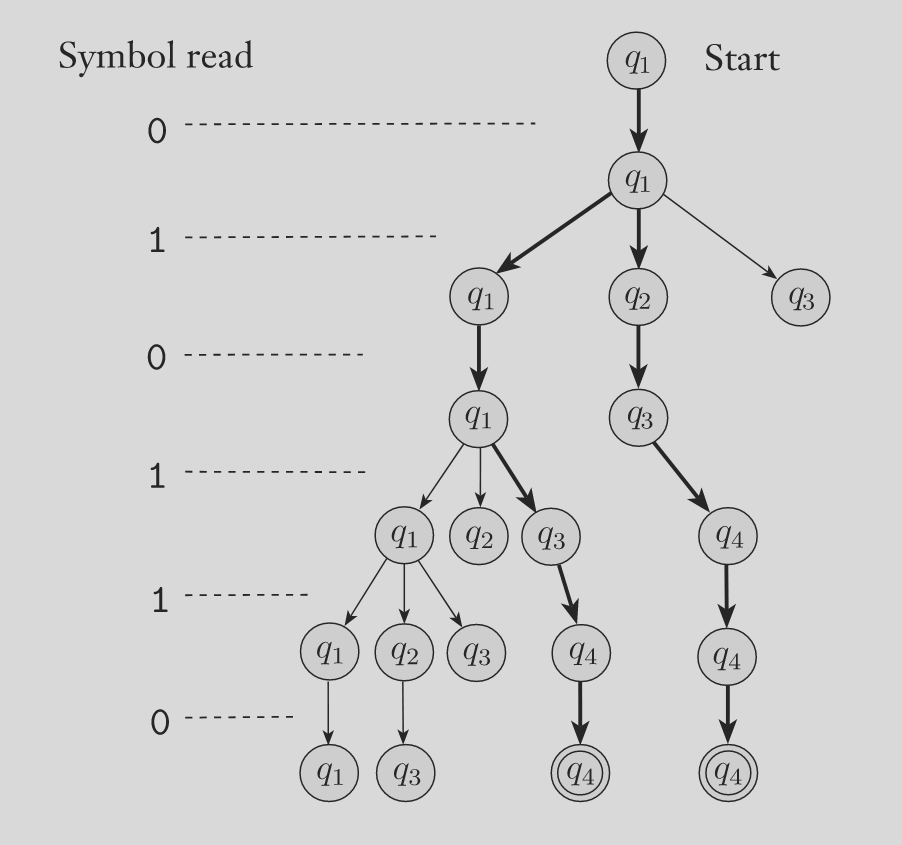
\includegraphics[scale=0.35]{../assets/nfa-neg.png}
            \caption{L'immagine rappresenta la computazione di $\ttt{010110}$ da parte di $N$.}
        \end{figure}

        \imp{Nota} nel momento in cui vengono incontrati $\varepsilon$-archi, si giunge allo stato successivo della computazione nello stesso step dell'input appena elaborato, senza produrre un passo ulteriore, producendo inoltre un nuovo ramo di computazione.
    \end{example}

    \begin{frameddefn}{Stringhe accettate (NFA)}
        Sia $N = (Q, \Sigma, \delta, q_0, F)$ un NFA, e sia $w = w_1\cdots w_n$ una stringa tale per cui $\forall i \in [1, n] \quad w_i \in \Sigma$; allora, $M$ \tbf{accetta} $w$ se esiste una sequenza di stati $r_0, \ldots, r_n \in Q$ tali per cui

        \begin{itemize}
            \item $r_0 = q_0$
            \item $\forall i \in [0, n - 1] \quad r_{i + 1} \in \delta(r_i, w_{i + 1})$
            \item $r_n \in F$
        \end{itemize}
    \end{frameddefn}

    \begin{frameddefn}{Equivalenza tra automi}
        Due macchine si dicono \tbf{equivalenti} se e solo se riconoscono lo stesso linguaggio.
    \end{frameddefn}

    \begin{framedthm}[label={nfa equiv}]{DFA equivalente ad NFA}
        Sia $N$ un NFA; allora, esiste un DFA ad esso equivalente. In simboli $$\mathcal{L}(\mathrm{NFA}) = \mathcal{L}(\mathrm{DFA})$$
    \end{framedthm}

    \begin{proof}
        Sia $N = (Q, \Sigma_{\varepsilon}, \delta, q_0, F)$ l'NFA in ipotesi, tale da riconoscere un linguaggio A. Inoltre, si definisca $$\forall k \ge 0 \quad \displaystyle E(R) := \bigcup_{r \in R}{\delta^k(r, \varepsilon)}$$ l'insieme degli stati raggiungibili da stati in $R$, applicando (anche ripetutamente) un numero arbitrario di $\varepsilon$-archi (si noti che per $k = 0$ si ha che $R \subseteq E(R)$).

        Allora, sia $M = (Q', \Sigma, \delta', q_0', F)$ il DFA definito come segue:

        \begin{itemize}
            \item $Q' := \powerset{(Q)}$, scelto tale da rappresentare ogni possibile stato di $N$;
            \item $\displaystyle \forall R \in Q', a \in \Sigma \quad \delta'(R, a) := \bigcup_{r \in R}{E(\delta(r, a))}$, scelta tale in quanto, per un certo insieme di stati $R \in Q'$ di $N$, a $\delta'(R, a)$ viene assegnata l'unione degli stati che sarebbero stati raggiunti in $N$ dagli $r \in R$ con $a$, calcolati dunque attraverso $\delta(r, a)$, aggiungendo infine i possibili $\varepsilon$-archi;
            \item $q_0' := E(\{q_0\})$, scelto tale da far iniziare $M$ esattamente dove aveva inizio $N$, comprendendo anche i possibili $\varepsilon$-archi iniziali;
            \item $F' := \{R \in Q' \mid \exists r \in R : r \in F\}$, che corrisponde all'insieme degli insiemi di stati di $N$ contenenti almeno uno stato accettante in $N$.
        \end{itemize}

        Allora $M$ è in grado di riconoscere $A$ per costruzione, poiché il DFA costruito emula l'NFA di partenza, tenendo anche in considerazione gli $\varepsilon$-archi. Dunque, sia $N$ che $M$ riconoscono $A$, e per definizione sono di conseguenza equivalenti.
    \end{proof}
    
    \begin{framedcor}[label={nfa regolare}]{Linguaggi regolari con NFA}
        Un linguaggio è regolare se e solo se esiste un NFA che lo riconosce.
    \end{framedcor}

    \proofiff{
        Sia $A$ un linguaggio regolare, e dunque per definizione esiste un DFA che lo riconosce. Allora, poiché un DFA è sempre anche NFA, segue la tesi.
    }{
        Sia $A$ un linguaggio tale da essere riconosciuto da un NFA; allora, per il \cref{nfa equiv}, esiste un DFA equivalente all'NFA che riconosce $A$, e dunque per definizione $A$ è regolare.
    }

    \section{Operazioni regolari}

    \subsection{Unione}
    
    \begin{frameddefn}{Unione}
        Siano $A$ e $B$ due linguaggi su un alfabeto $\Sigma$; allora, si definisce l'\tbf{unione} di $A$ e $B$ il seguente linguaggio: $$A \cup B := \{x \mid x \in A \lor x \in B \}$$
    \end{frameddefn}

    \begin{example}[Unione]
        Sia $\Sigma = \{\ttt a , \ldots, \ttt z\}$ l'alfabeto composto da 26 lettere, e siano $A = \{\ttt{uno}, \ttt{due}\}$ e $B = \{\ttt{tre}, \ttt{quattro}\}$ due linguaggi su $\Sigma$. Allora, si ha che $$A \cup B = \{\ttt{uno}, \ttt{due}, \ttt{tre}, \ttt{quattro}\}$$
    \end{example}

    \begin{framedprop}[label={closure unione}]{Chiusura dell'unione}
        Siano $A$ e $B$ due linguaggi regolari su un alfabeto $\Sigma$; allora $A \cup B$ è regolare.
    \end{framedprop}

    \begin{proof}[Dimostrazione I]
        Per definizione, $A$ e $B$ sono linguaggi regolari, dunque esistono due automi finiti $$\left. \begin{array}{c}M_1 = (Q_1, \Sigma, \delta_1, q_1, F_1) \\ M_2 = (Q_2, \Sigma, \delta_2, q_2, F_2)\end{array} \right.$$ tali da riconoscere rispettivamente $A$ e $B$. Allora, sia $M = (Q, \Sigma, \delta, q_0, F)$ l'automa finito definito come segue:

        \begin{itemize}
            \item $Q := Q_1 \times Q_2 = \{(r_1, r_2) \mid r_1 \in Q_1 \land r_2 \in Q_2\}$, scelto tale in quanto permette di avere tutte le possibili combinazioni di stati dei due automi di partenza;
            \item $\forall (r_1, r_2) \in Q, a \in \Sigma \quad \delta((r_1, r_2), a) := (\delta_1(r_1, a), \delta_2(r_2, a))$, scelta tale in quanto permette di simulare entrambi gli automi di partenza contemporaneamente, mandando ogni stato di $M_1$ ed $M_2$ dove sarebbe andato nei rispettivi automi di appartenenza;
            \item $q_0 := (q_1, q_2)$, scelto tale in quanto deve essere lo stato in cui entrambe gli automi in ipotesi iniziavano;
            \item $F := (F_1 \times Q_2) \cup (Q_1 \times F_2) = \{(r_1, r_2) \mid r_1 \in F_1 \lor r_2 \in F_2\}$, scelto tale in quanto permette di simulare gli stati accettanti di entrambi gli automi, e vanno prese tutte le coppie che vedono almeno uno dei due stati come accettanti poiché altrimenti non si accetterebbero delle stringhe accettate da $M_1$ ed $M_2$ in partenza.
        \end{itemize}

        Allora, poiché $M$ è in grado di simulare $M_1$ ed $M_2$ contemporaneamente, per costruzione accetterà ogni stringa di $A$ e di $B$, dunque riconoscendo $A \cup B$, e di conseguenza $A \cup B$ è regolare per definizione.
    \end{proof}

    \begin{proof}[Dimostrazione II]
        Per definizione, $A$ e $B$ sono linguaggi regolari, dunque per il \cref{nfa equiv} esistono due NFA $$\left. \begin{array}{c}N_1 = (Q_1, \Sigma, \delta_1, q_1, F_1) \\ N_2 = (Q_2, \Sigma, \delta_2, q_2, F_2) \end{array} \right.$$ tali da riconoscere rispettivamente $A$ e $B$. Allora, sia $N = (Q, \Sigma, \delta, q_0, F)$ l'NFA costruito come segue:

        \begin{itemize}
            \item $Q := \{q_0\} \cup Q_1 \cup Q_2$, dove $q_0$ è un nuovo stato, e $Q$ è scelto tale da includere sia $N_1$ che $N_2$;
            \item $\forall q \in Q, a \in \Sigma_{\varepsilon} \quad \delta(q, a) := \left \{ \begin{array}{ll} \delta_1(q, a) & q \in Q_1 \\ \delta_2(q, a) & q \in Q_2 \\ \{q_1, q_2\} & q = q_0 \land a = \varepsilon \\ \emptyset & q = 0 \land a \neq \varepsilon \end{array} \right.$, scelta tale da poter eseguire contemporaneamente gli NFA $N_1$ ed $N_2$, definendo per casi la funzione di transizione; infatti, si noti che si è posta $\delta(q_0, \varepsilon) := \{q_1, q_2\}$ in modo da collegare il nuovo stato $q_0$ a $q_1$ e $q_2$, gli stati iniziali di $N_1$ ed $N_2$ rispettivamente;
            \item $q_0$ è il nuovo stato, che rappresenta lo stato iniziale di $N$;
            \item $F := F_1 \cup F_2$, scelto tale da costruire $N$ in modo che accetti una stringa se e solo se la accetterebbero $N_1$ o $N_2$.
        \end{itemize}

        Allora, l'NFA risultante $N$ è in grado di computare contemporaneamente $N_1$ ed $N_2$, ed è dunque in grado di riconoscere $A$ e $B$ contemporaneamente; di conseguenza, $N$ riconosce $A \cup B$, che risulta dunque essere regolare per definizione.

        \begin{figure}[H]
            \centering
            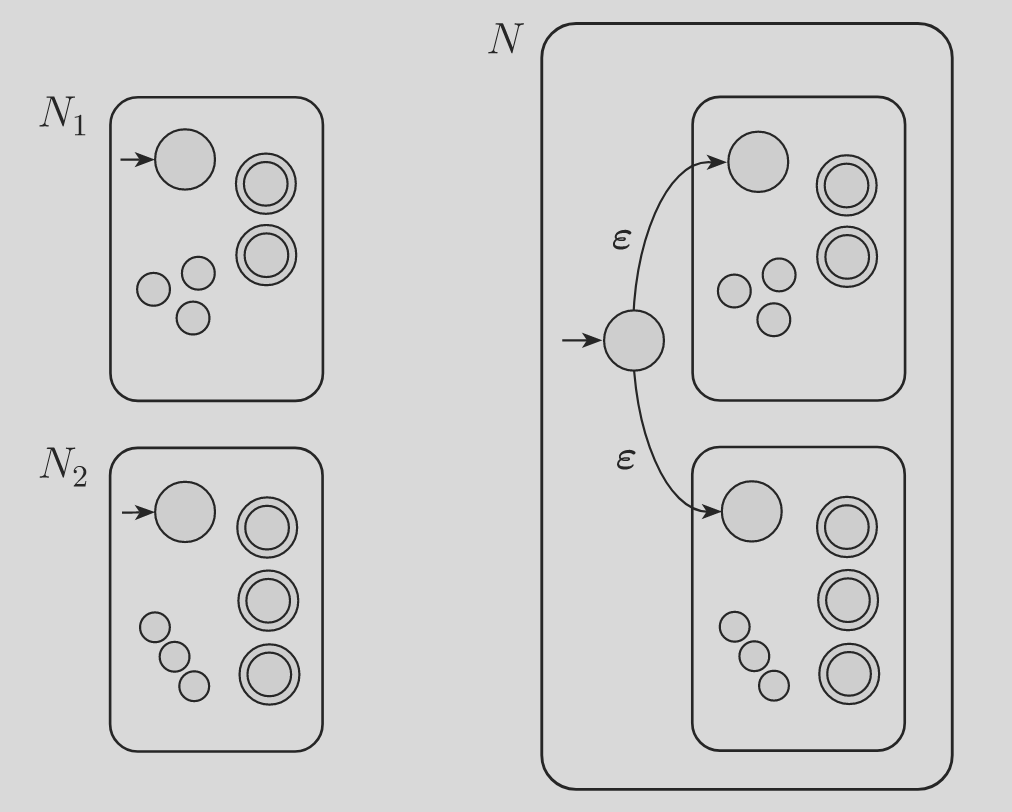
\includegraphics[scale=0.35]{../assets/union-neg.png}
            \caption{L'immagine raffigura la dimostrazione costruttiva descritta.}
        \end{figure}

    \end{proof}

    \subsection{Intersezione}

    \begin{frameddefn}{Intersezione}
        Siano $A$ e $B$ due linguaggi su un alfabeto $\Sigma$; allora, si definisce l'\tbf{intersezione} di $A$ e $B$ il seguente linguaggio: $$A \cap B := \{x \mid x \in A \land x \in B \}$$
    \end{frameddefn}

    \begin{example}[Intersezione]
        Sia $\Sigma = \{\ttt a , \ldots, \ttt z\}$ l'alfabeto composto da 26 lettere, e siano $A = \{\ttt{uno}, \ttt{due}\}$ e $B = \{\ttt{uno}, \ttt{tre}\}$ due linguaggi su $\Sigma$. Allora, si ha che $$A \cap B = \{\ttt{uno}\}$$
    \end{example}

    \begin{framedprop}{Chiusura dell'intersezione}
        Siano $A$ e $B$ due linguaggi regolari su un alfabeto $\Sigma$; allora $A \cap B$ è regolare.
    \end{framedprop}

    \begin{proof}
        TODO
    \end{proof}

    \subsection{Concatenazione}

    \begin{frameddefn}{Concatenazione}
        Siano $A$ e $B$ due linguaggi su un alfabeto $\Sigma$; allora, si definisce la \tbf{concatenazione} di $A$ e $B$ il seguente linguaggio: $$A \circ B = \{xy \mid x \in A \land y \in B\}$$ Si noti che per ogni linguaggio $L$ è vero che $\emptyset \circ L = L \circ \emptyset = \{ \varepsilon \} \circ L = L \circ \{ \varepsilon \} = L$.
    \end{frameddefn}

    \begin{example}[Concatenazione]
        Sia $\Sigma = \{\ttt a , \ldots, \ttt z\}$ l'alfabeto composto da 26 lettere, e siano $A = \{\ttt{uno}, \ttt{due}\}$ e $B = \{\ttt{tre}, \ttt{quattro}\}$ due linguaggi su $\Sigma$. Allora, si ha che $$A \circ B := \{\ttt{unotre}, \ttt{unoquattro}, \ttt{duetre}, \ttt{duequattro}\}$$
    \end{example}

    \begin{framedprop}[label={closure concat}]{Chiusura della concatenazione}
        Siano $A$ e $B$ due linguaggi regolari su un alfabeto $\Sigma$; allora $A \circ B$ è regolare.
    \end{framedprop}

    \begin{proof}
        Per definizione, $A$ e $B$ sono linguaggi regolari, dunque per il \cref{nfa equiv} esistono due NFA $$\left. \begin{array}{c}N_1 = (Q_1, \Sigma, \delta_1, q_1, F_1) \\ N_2 = (Q_2, \Sigma, \delta_2, q_2, F_2) \end{array} \right.$$ tali da riconoscere rispettivamente $A$ e $B$. Allora, sia $N = (Q, \Sigma, \delta, q_0, F)$ l'NFA costruito come segue:
        
        \begin{itemize}
            \item $Q := Q_1 \cup Q_2$, scelto tale da includere entrambe gli automi $N_1$ ed $N_2$ di partenza;
            \item $q_0 := q_1$, scelto tale da far iniziare l'esecuzione dell'automa su $N_1$;
            \item $F := F_2$, scelto tale da far terminare l'esecuzione dell'automa su $N_2$;
            \item $\forall q \in Q, a \in \Sigma_\varepsilon \quad \delta(q, a) := \left \{ \begin{array}{ll} \delta_1(q, a) & q \in Q_1 - F_1 \lor (q \in F_1 \land a \neq \varepsilon) \\ \delta_1(q, a) \cup \{q_2\} & q \in F_1 \land a = \varepsilon \\ \delta_2(q, a) & q \in Q_2 \end{array} \right.$, scelta tale da anteporre l'esecuzione di $N_1$ a quella di $N_2$; infatti, se $q \in Q_1 - F_1$ (è uno stato non accettante di $N_1$), oppure $q \in F_1$ ma $a \neq \varepsilon$, l'esecuzione di $N_1$ non viene alterata; diversamente, se invece $q \in F_1$ e $a = \varepsilon$, all'insieme di stati $\delta_1(q, \varepsilon)$ viene aggiunto $q_2$, ovvero lo stato iniziale di $N_2$, in modo da effettuare la concatenazione tra i due NFA non deterministicamente.
        \end{itemize}

        Allora, l'NFA $N$ costruito computa inizialmente $N_1$, e se vengono raggiunti suoi stati accettanti, l'esecuzione prosegue attraverso $N_2$, al fine di realizzare la concatenazione tra le stringhe. Di conseguenza, l'automa è in grado di riconoscere $A \circ B$ per costruzione, e dunque $A \circ B$ è regolare per definizione.

        \begin{figure}[H]
            \centering
            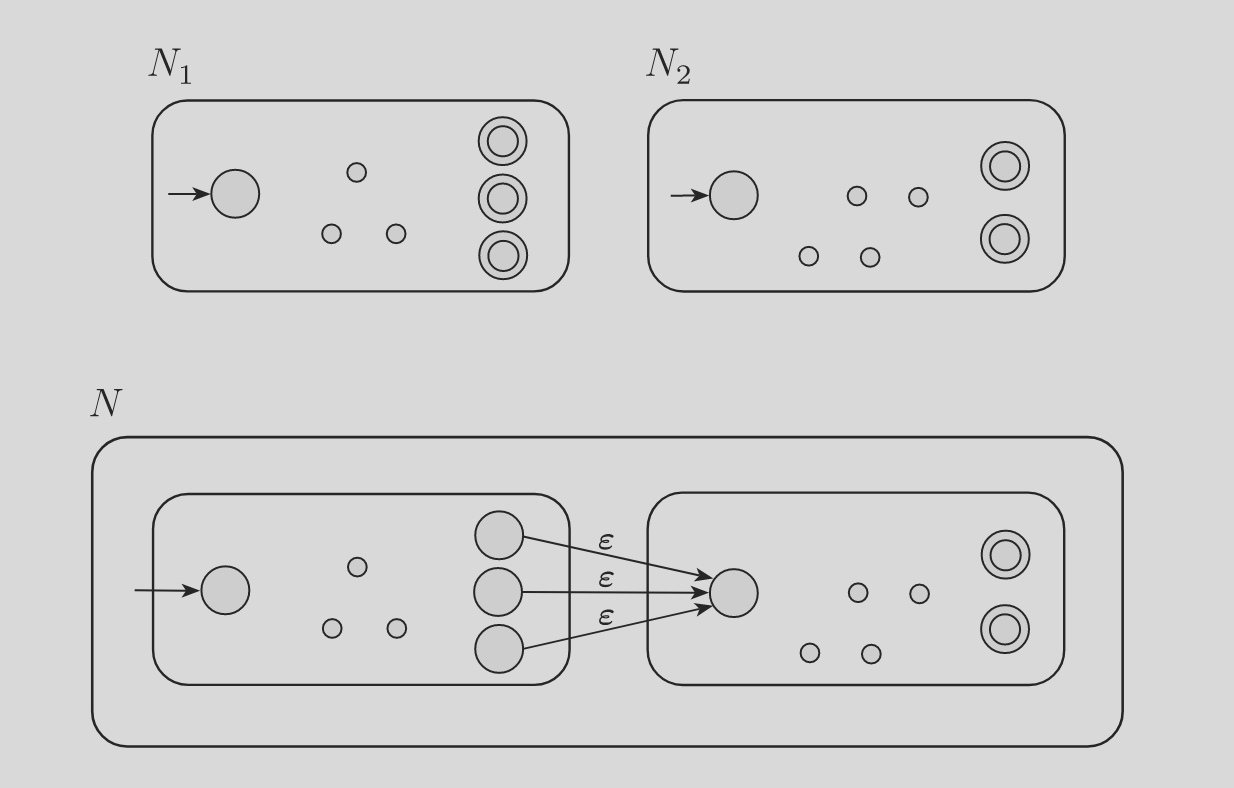
\includegraphics[scale=0.35]{../assets/concat-neg.png}
            \caption{L'immagine raffigura la dimostrazione costruttiva descritta.}
        \end{figure}
    \end{proof}

    \begin{frameddefn}{Elevamento a potenza}
        Sia $A$ un linguaggio; allora, si definisce \tbf{elevamento a potenza} di $A$ il seguente linguaggio: $$A^n := \underbrace{A \circ \cdots \circ A}_{n \ \textrm{volte}} = \soe{ll}{A^0 := \{\varepsilon \} & \\ A^n = A^{n -1} \circ A & n \ge 1}$$
    \end{frameddefn}

    \begin{example}[Elevamento a potenza]
        Sia $\Sigma = \{\ttt a , \ldots, \ttt z\}$ l'alfabeto composto da 26 lettere, e sia $A = \{\ttt{uno}, \ttt{due}\}$ un linguaggio su $\Sigma$. Allora, si ha che $$A^2 = \{\varepsilon, \ttt{uno}, \ttt{due}, \ttt{unouno}, \ttt{unodue}, \ttt{dueuno}, \ttt{duedue}\}$$
    \end{example}

    \subsection{Star}

    \begin{frameddefn}{Star}
        Sia $A$ un linguaggio; allora, si definisce l'operazione unaria \tbf{star} che definisce il seguente linguaggio: $$A^* := \{x_1 \cdots x_k \mid k \ge 0 \land \forall i \in [1, k] \quad x_i \in A\} = \displaystyle \bigcup_{n \in \N}{L^n}=\{ \varepsilon \} \cup L \cup L^2 \cup \ldots$$

        Si noti che $k = 0 \implies \varepsilon \in A^*$ per ogni linguaggio $A$.
    \end{frameddefn}

    \begin{example}[Star]
        Sia $\Sigma = \{\ttt a , \ldots, \ttt z\}$ l'alfabeto composto da 26 lettere, e sia $A = \{\ttt{uno}, \ttt{due}\}$ un linguaggio su $\Sigma$. Allora, si ha che $$A^* := \{\varepsilon, \ttt{uno}, \ttt{due}, \ttt{unouno}, \ttt{unodue}, \ttt{dueuno}, \ttt{duedue}, \ldots\}$$
    \end{example}
   
    \begin{example}[Stringhe binarie]
        Si noti che nel caso di $\Sigma = \{ \ttt 0, \ttt 1 \}$, si ha che $\Sigma^*$ è l'insieme di ogni stringa binaria, di arbitraria lunghezza.
    \end{example}

    \begin{framedprop}[label={closure star}]{Chiusura dell'operazione star}
        Sia $A$ un linguaggio regolare su un alfabeto $\Sigma$; allora $A^*$ è regolare.
    \end{framedprop}

    \begin{proof}
        Per definizione, $A$ è linguaggio regolare, dunque per il \cref{nfa equiv} esiste un NFA $$N_1 = (Q_1, \Sigma, \delta_1, q_1, F_1)$$ tale da riconoscere $A$. Allora, sia $N = (Q, \Sigma, \delta, q_0, F)$ l'NFA costruito come segue:

        \begin{itemize}
            \item $Q := \{q_0\} \cup Q_1$, dove $q_0$ è un nuovo stato, posto prima di $N_1$;
            \item $q_0$ è il nuovo stato iniziale;
            \item $F: = \{q_0\} \cup F_1$, poiché $q_0$ deve essere accettante, in modo tale da accettare $\varepsilon$ (si noti che $\varepsilon \in A^*$ per ogni linguaggio $A$);
            \item $\forall q \in Q, a \in \Sigma_\varepsilon \quad \delta(q, a) := \left \{ \begin{array}{ll} \delta_1(q, a) & q \in Q_1 - F_1 \lor (q \in F_1 \land a \neq \varepsilon) \\ \delta_1(q, a) \cup \{q_1\} & q \in F_1 \land a = \varepsilon \\ \{q_1\} & q = q_0 \land a = \varepsilon \\ \emptyset & q = q_0 \land a \neq \varepsilon \end{array} \right.$, scelta tale da ricominciare l'esecuzione dell'automa ogni volta che viene raggiunto uno stato accettante in $N_1$; infatti, se $q \in Q_1 - F_1$ (è uno stato non accettante di $N_1$), oppure $q$ è accettante e $a \neq \varepsilon$, l'esecuzione procede normalmente con $\delta_1(q, a)$; differentemente, se $q \in F_1$ ma $a = \varepsilon$, allora l'esecuzione deve ricominciare da capo per poter effettuare la concatenazione multipla delle stringhe in $A$ che caratterizzano l'operazione star, e dunque a $\delta_1(q, a)$ viene aggiunto $q_1$ (lo stato inziale di $N_1$); infine, ponendo $\delta(q_0, \varepsilon) := \{q_1\}$ si realizza l'$\varepsilon$-arco iniziale che collega $q_0$ (il nuovo stato) a $q_1$, al fine di rendere $N$ in grado di accettare $\varepsilon$.
        \end{itemize}

        Allora, poichè l'NFA $N$ è in grado di ricominciare l'esecuzione ogni volta che questa sarebbe terminata in $N_1$, è in grado di accettare molteplici copie concatenate delle stringhe in $A$, in maniera non deterministica, e dunque per definizione $N$ riconosce $A^*$, il quale risulta allora essere regolare per definizione.

        \begin{figure}[H]
            \centering
            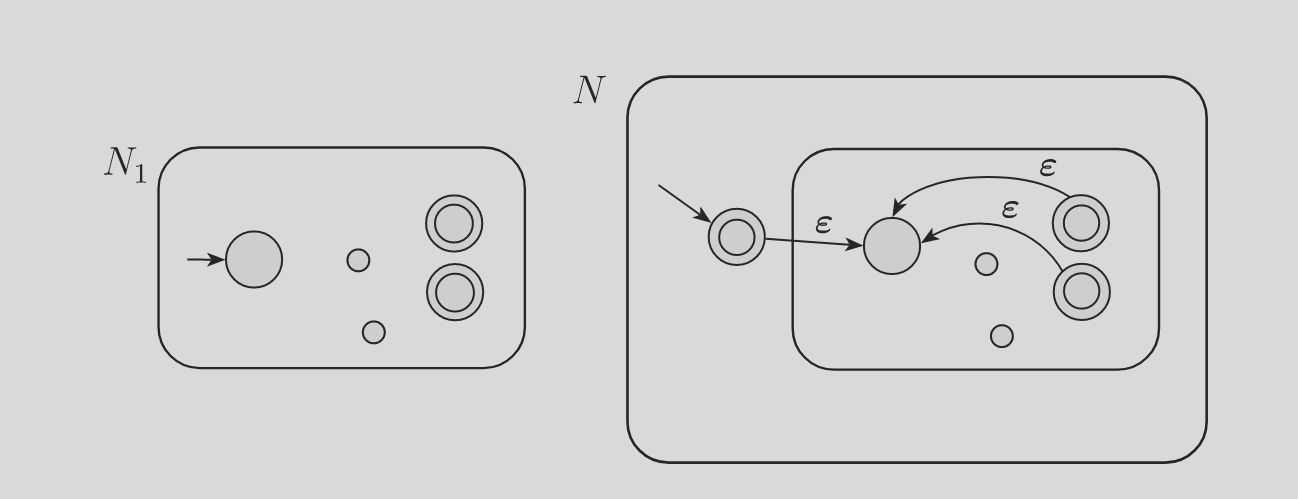
\includegraphics[scale=0.35]{../assets/star-neg.png}
            \caption{L'immagine raffigura la dimostrazione costruttiva descritta.}
        \end{figure}
    \end{proof}

    \subsection{Complemento}

    \begin{frameddefn}{Complemento}
        Sia $A$ un linguaggio definito su un alfabeto $\Sigma$; allora si definisce il \tbf{complemento} di $A$ il seguente linguaggio: $$\lnot A := \{x \mid x \notin A\}$$
    \end{frameddefn}

    \begin{example}[Complemento]
        Sia $\Sigma = \{\ttt 0, \ttt 1\}$ l'alfabeto binario, e sia $A = \{ \ttt{00}, \ttt{1}\}$ un linguaggio definito su di esso. Allora il suo complemento è il seguente: $$\lnot A = \{\varepsilon, \ttt 0, \ttt 1, \ttt{01}, \ttt{10}, \ttt{000}, \ldots\}$$
    \end{example}

    \begin{framedprop}{Chiusura del complemento}
        Sia $A$ un linguaggio regolare su un alfabeto $\Sigma$; allora $\lnot A$ è regolare.
    \end{framedprop}

    \begin{proof}
        TODO
    \end{proof}

    \begin{frameddefn}{Leggi di De Morgan}
        Siano $A$ e $B$ definiti su un alfabeto $\Sigma$; allora, sono vere le seguenti, che prendono il nome di \tbf{leggi di De Morgan}:

        \begin{enumerate}[label=\roman*), font=\itshape]
            \item $\lnot (A \cup B) = \lnot A \cap \lnot B$
            \item $\lnot (A \cap B) = \lnot A \cup \lnot B$
        \end{enumerate}
    \end{frameddefn}

    \section{Espressioni regolari}

    \subsection{Definizioni}

    \begin{frameddefn}{Espressione regolare}
        Sia $\Sigma$ un alfabeto; allora, $R$ si definisce \tbf{espressione regolare} se soddisfa una delle seguenti caratteristiche:

        \begin{itemize}
            \item $R = \emptyset$
            \item $R = \varepsilon$
            \item $R \in \Sigma$
        \end{itemize}

        Un'espressione regolare, dunque, è un modo compatto di definire un linguaggio. Si noti che le definizioni successive sono in grado di espandere la definizione appena fornita. L'insieme di tutte le espressioni su $\Sigma$ è denotato con $\mathcal{R}$.

        Data un'espressione regolare $R$, con $L(R)$ si intende il linguaggio che $R$ descrive, ovvero l'insieme di stringhe che $R$ rappresenta. Dunque, sono vere le seguenti:

        \begin{itemize}
            \item $L(\emptyset) = \emptyset$
            \item $L(\varepsilon) = \{ \varepsilon \}$
            \item $\forall a \in \Sigma \quad L(a) = \{ a\}$
        \end{itemize}
    \end{frameddefn}

    \begin{frameddefn}{Unione}
        Siano $R_1$ ed $R_2$ due espressioni regolari; allora, si definisce l'\tbf{unione} di $R_1$ ed $R_2$ la seguente espressione regolare: $$(R_1 \cup R_2)$$ e rappresenta uno qualsiasi dei caratteri di $R_1$ o di $R_2$.

        Si noti che $R \cup \emptyset = \emptyset$ per qualsiasi espressione regolare $R$.
    \end{frameddefn}

    \begin{example}[Unione]
        Sia $\Sigma = \{\ttt a, \ttt b, \ttt c\}$ un alfabeto; un esempio di espressione regolare di unione su $\Sigma$ è il seguente: $$R = (\ttt a \cup \ttt c)$$ ed il valore di questa espressione equivale da $\ttt a$ oppure $\ttt c$, e dunque $L(R) = \{ \ttt a, \ttt c\}$.
    \end{example}

    \begin{example}[Espressioni regolari particolari]
        Sia $\Sigma = \{\ttt 0, \ttt 1\}$ un alfabeto; l'espressione regolare $(\ttt 0 \cup \ttt 1)$ rappresenta il linguaggio che consiste di tutte le stringhe di lunghezza 1 sull'alfabeto $\Sigma$, e dunque l'espressione regolare descritta si abbrevia generalmente con il simbolo $\Sigma$ stesso.
    \end{example}

    \begin{frameddefn}{Concatenazione}
        Siano $R_1$ ed $R_2$ due espressioni regolari; allora, si definisce la \tbf{concatenazione} di $R_1$ ed $R_2$ la seguente espressione regolare: $$(R_1 \circ R_2)$$ e rappresenta le stringhe che iniziano per $R_1$ e terminano con $R_2$.

        Per indicare la concatenazione di $R$ con sé stessa, si usa la seguente notazione $$R^k := \underbrace{R \circ \cdots \circ R}_{k \ \textrm{volte}}$$

        Si noti che $R \circ \emptyset = \emptyset$ e $R \circ \varepsilon = R$, per qualsiasi espressione regolare $R$.
    \end{frameddefn}

    \begin{example}[Concatenazione]
        Sia $\Sigma = \{\ttt a, \ttt b, \ttt c\}$ un alfabeto; un esempio di espressione regolare di concatenazione su $\Sigma$ è il seguente: $$R = (\ttt a \circ \ttt c)$$ che può essere scritto equivalentemente come $\ttt a \ttt c$, e dunque $L(R) = \{ \ttt{ac} \}$.
    \end{example}

    \begin{frameddefn}{Star}
        Sia $R$ un'espressione regolare; allora, si definisce l'operazione unaria \tbf{star} su $R$ la seguente espressione regolare: $$(R^*)$$ e tutte rappresenta le stringhe che si possono ottenere concatenando un qualsiasi numero di caratteri di $R$, e descrive dunque il linguaggio che consiste di tutte le stringhe dell'alfabeto di $R$.

        Si noti che $R^*$ comprende $\varepsilon$ per qualsiasi espressione regolare $R$.

        Spesso si usa la notazione $R^+ := RR^*$, ovvero le stringhe che si ottengono attraverso la concatenazione di 1 o più stringhe di $R$. Di conseguenza, si ha che $R^+ \cup \varepsilon = R^*$.
    \end{frameddefn}

    \begin{example}[Star]
        Sia $\Sigma = \{\ttt a, \ttt b, \ttt c\}$ un alfabeto; un esempio di espressione regolare di star su $\Sigma$ è il seguente: $$R = (\Sigma^*)$$ che descrive il linguaggio che consiste di tutte le stringhe possibili sull'alfabeto, e dunque $$L(R) = \{\varepsilon, \ttt a, \ttt b, \ttt c, \ttt{aa}, \ttt{bb}, \ttt{cc}, \ldots\}$$
    \end{example}

    \begin{example}[Espressioni regolari]
        Sia $\Sigma = \{\ttt 0, \ttt 1\}$ un alfabeto; i seguenti sono esempi di espressioni regolari su $\Sigma$:
        
        \begin{itemize}
            \item $L(\ttt 0 ^* \ttt 1 \ttt 0 ^*) = \{w \mid w$ contiene un solo $\ttt 1 \}$;
            \item $L(\Sigma ^* \ttt{001} \Sigma ^*) = \{ w \mid w$ contiene la stringa $\ttt{001}$ come sottostringa$\}$;
            \item $L(\ttt 0 \Sigma ^* \ttt 0 \cup \ttt 1 \Sigma ^* \ttt 1 \cup \ttt 0 \cup \ttt 1) = \{w \mid w$ inizia e termina con lo stesso carattere$\}$, poiché si noti che l'ordine delle operazioni, a meno di parentesi, è (\tit i) star, (\tit{ii}) concatenazione, ed infine (\tit{iii}) unione;
            \item $L((\ttt 0 \cup \varepsilon) (\ttt 1 \cup \varepsilon)) = \{\varepsilon, \ttt 0, \ttt 1, \ttt{01}\}$;
            \item $L(\emptyset ^*) = \{ \varepsilon \}$, poiché $\emptyset$ rappresenta il linguaggio vuoto, e dunque l'unica stringa che si può ottenere concatenando un qualsiasi numero di volte elementi del linguaggio vuoto, è $\varepsilon$.
        \end{itemize}
    \end{example}

    \section{Configurazioni}

    \subsection{Configurazioni di DFA}

    \begin{frameddefn}[label={extended trans}]{Estensione di $\delta$ dei DFA}
        Sia $M = (Q, \Sigma, \delta, q_0, F)$ un DFA; è possibile estendere la definizione della funzione di transizione $\delta$, utilizzando la notazione dell'operazione star, mediante la seguente definizione ricorsiva:

        \begin{equation*}
            \resizebox{.98\hsize}{!}{
                $\forall q \in Q, x \in \Sigma^* \quad \delta^*: Q \times \Sigma ^* \to Q : (q, x) \mapsto \soe{ll}{\delta^*(q, \varepsilon) = \delta(q, \varepsilon) & \\ \delta^*(q, by) =  \delta^*(\delta(q, b), y) & b \in \Sigma, y \in \Sigma^* \mid x = by}$
            }
        \end{equation*}
        
        Si noti che tale funzione prende in input uno stato ed una stringa, e restituisce lo stato in cui il DFA si troverà al termine della lettura dell'intera stringa di input. La notazione $\delta^*$ è coerente con la definizione dell'operazione star, poiché viene calcolata la transizione di stati attraverso $\delta$ fintanto che l'input non è stato esaurito.
    \end{frameddefn}

    \begin{frameddefn}{Configurazione di un DFA}
        Sia $M = (Q, \Sigma, \delta, q_0, F)$ un DFA; una tupla $(q, x) \in Q \times \Sigma^*$ è detta \tbf{configurazione} di M se $q$ è pari allo stato attuale della computazione di un certo input, ed $x$ è la porzione di input rimanente da leggere.
    \end{frameddefn}

    \begin{frameddefn}[label={rel config}]{Relazione tra configurazioni}
        Sia $M = (Q, \Sigma, \delta, q_0, F)$ un DFA, e siano $(p, x), (q, y) \in Q \times \Sigma^*$ due sue configurazioni durante la computazione di un certo input; allora, tali due configurazioni si dicono essere \tbf{in relazione} se e solo se dall'una è possibile passare all'altra. In simboli: $$(p, x) \vdash_M (q, y) \iff \soe{l}{p, q \in Q \\ x, y \in \Sigma^* \\ \exists a \in \Sigma \mid x = ay \land \delta(p, a) = q}$$
    \end{frameddefn}

    \begin{framedobs}{Chiusura transitiva di $\vdash$}
        Sia $M = (Q, \Sigma, \delta, q_0, F)$ un DFA; si noti che la chiusura transitiva della relazione tra configurazioni $\vdash$, ovvero $\vdash^*$, equivale a calcolare gli input attraverso la funzione di transizione estesa $\delta^*$ definita nella \cref{extended trans}.
    \end{framedobs}

    \begin{example}[Chiusura transitiva di $\vdash$]
        Sia $M = (Q, \sigma, \delta, q_0, F)$ un DFA, e sia $(p, x) \in Q \times \Sigma ^*$ una sua configurazione durante la computazione di un certo input; inoltre, siano $a, b, c \in \Sigma$ tali che $x = abc$. Inoltre, siano vere le seguenti:

        \begin{itemize}
            \item $(p, abc) \vdash_M (p_1, bc)$
            \item $(p_1, bc) \vdash_M (p_2, c)$
            \item $(p_2, c) \vdash_M (q, \varepsilon)$
        \end{itemize}

        per certi $p, p_1, p_2, q \in Q$; allora, si ha che $(p, x) \vdash_M^* (q, \varepsilon)$, poiché è possibile raggiungere lo stato $q$, partendo da $p$, attraverso l'input $x = abc$.
    \end{example}

    \begin{framedobs}{Determinismo}
        Dato un DFA $M = (Q, \Sigma, \delta, q_0, F)$, è possibile fornire una definizione di \tit{determinismo} alternativa, attraverso la relazione tra configurazioni definita nella \cref{rel config}, come segue: $$\forall q \in Q, a \in \Sigma, x \in \Sigma ^* \quad \exists ! p \in Q \mid (q, ax) \vdash_M (p, x)$$
    \end{framedobs}

    \subsection{Configurazioni di NFA}

    TODO

    \begin{framedobs}{Linguaggio di un automa}
        Dato un automa $M$, la \cref{def L(M)} si può riscrivere in simboli come segue: $$L(M) := \{x \in \Sigma ^* \mid \delta^*(q_0, x) \in F \iff \exists q \in F \mid (q_0, x) \vdash_M^* (q, \varepsilon)\}$$

        Si noti che, nella definizione, verrà presa in considerazione la funzione $\delta^*$ corrispondente alla classe dell'automa $M$ in questione.
    \end{framedobs}

    \section{Non determinismo generalizzato}

    \subsection{Definizioni}
    
    \begin{frameddefn}[label={def gnfa}]{GNFA}
        Un \tbf{GNFA} (\tit{Generalized Nondeterministic Finite Automaton}) è una versione generalizzata di un NFA, in cui gli archi delle transizioni sono espressioni regolari sull'alfabeto dato.

        Un GNFA legge blocchi di simboli dall'input, e si muove lungo gli archi che sono etichettati da espressioni regolari che possono descrivere il blocco di simboli letto.

        Inoltre, essendo una versione generalizzata di un NFA, un GNFA può avere diversi modi di elaborare la stessa stringa di input, e accetta quest'ultima se la sua elaborazione può far si che il GNFA si trovi in uno stato accettante al suo termine.

        \imp{Nota} All'interno di questi appunti, a meno di specifica, si assume che ogni GNFA preso in considerazione abbia:

        \begin{itemize}
            \item un solo stato di inizio, privo di archi entranti, connesso con ogni altro stato, ma non con sé stesso;
            \item un solo stato accettante, privo di archi uscenti, non connesso con altri archi;
            \item ogni altro stato collegato con ogni altro stato, a meno di quello iniziale, anche con sé stessi.
        \end{itemize}

        Formalmente, dato un alfabeto $\Sigma$, un GNFA del tipo appena descritto è una quintupla $(Q, \Sigma, \delta, q_{\mathrm{start}}, q_{\mathrm{accept}})$ definita come segue:

        \begin{itemize}
            \item $Q$ è l'\textbf{insieme degli stati} dell'automa, un insieme \textit{finito}
            \item $\Sigma$ è l'\textbf{alfabeto dell'automa}, un insieme \textit{finito}
            \item $\func{\delta}{(Q - \{q_{\mathrm{accept}}\}) \times (Q - \{q_{\mathrm{start}}\})}{\mathcal{R}}$ è la \textbf{funzione di transizione}, che definisce la relazione tra gli stati; si noti che $\delta$ ha come dominio il prodotto cartesiano tra gli stati, e come codominio $\mathcal{R}$, poiché a differenza di un normale DFA o NFA, un GNFA prende come input 2 stati (che non possono essere né quello iniziale né quello accettante) e restituisce un'espressione regolare
            \item $q_{\mathrm{start}} \in Q$ è lo \textbf{stato iniziale}
            \item $q_{\mathrm{accept}}$ è lo \textbf{stato accettante}
        \end{itemize}
    \end{frameddefn}

    \begin{example}[GNFA]
        Il seguente è il digramma di un GNFA sull'alfabeto $\Sigma = \{ \ttt a, \ttt b \}.$

        \begin{figure}[H]
            \centering
            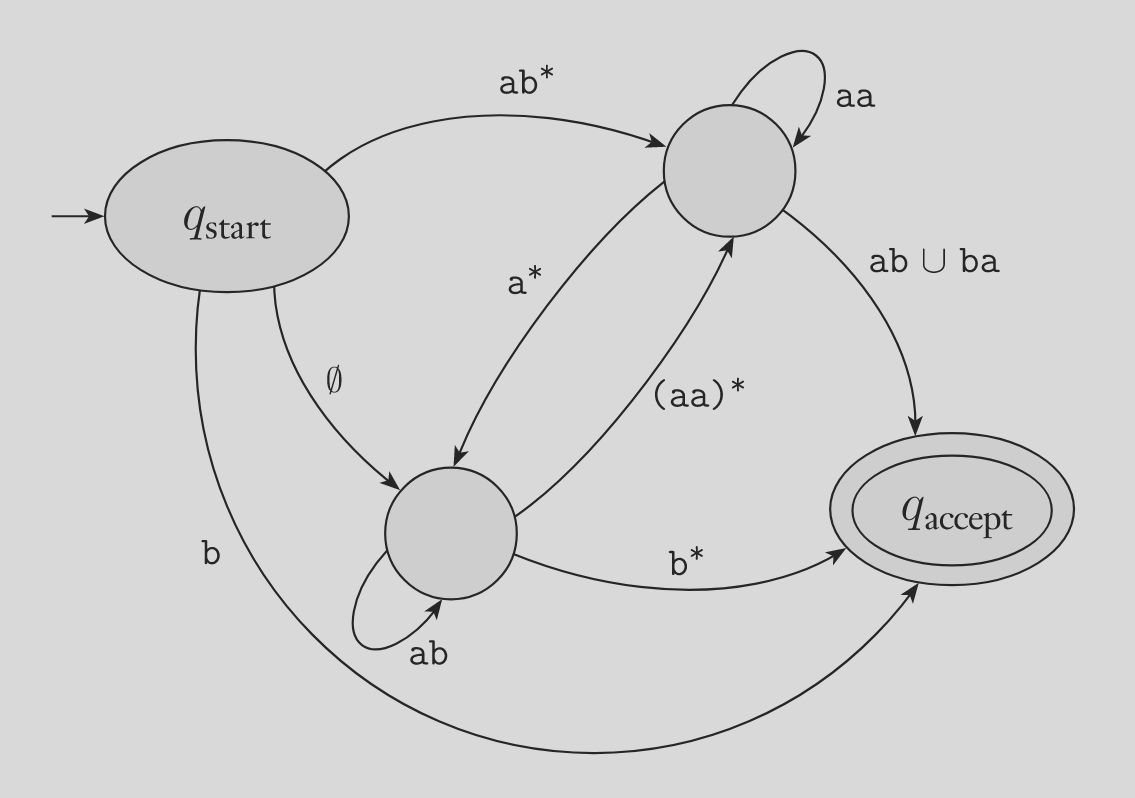
\includegraphics[scale=0.3]{../assets/gnfa-neg.png}
            \caption{Un GNFA.}
        \end{figure}
    \end{example}

    \begin{frameddefn}{Stringhe accettate (GNFA)}
        Sia $G = (Q, \Sigma, \delta, q_{\mathrm{start}}, q_{\mathrm{accept}})$ un GNFA, e sia $w = w_1\cdots w_n$ una stringa tale per cui $\forall i \in [1, n] \quad w_i \in \Sigma^*$; allora, $G$ \tbf{accetta} $w$ se esiste una sequenza di stati $q_0, \ldots, q_n \in Q$ tali per cui

        \begin{itemize}
            \item $q_0 = q_{\mathrm{start}}$
            \item $\forall i \in [0, n - 1] \quad w_i \in L(\delta(q_i, q_{i + 1}))$, ovvero, $w_i$ deve far parte del linguaggio rappresentato dall'espressione regolare sull'arco da $q_i$ a $q_{i + 1}$
            \item $q_n = q_{\mathrm{accept}}$
        \end{itemize}
    \end{frameddefn}

    \begin{framedmeth}[label={dfa into gnfa}]{GNFA di un DFA}
        Sia $M$ un DFA; allora per costruire un GNFA ad esso equivalente, è sufficiente:

        \begin{itemize}
            \item aggiungere un nuovo stato iniziale, con un $\varepsilon$-arco entrante sul vecchio stato iniziale;
            \item aggiungere un nuovo stato accettante, con $\varepsilon$-archi entranti provenienti dai vecchi stati accettanti;
            \item per gli archi con etichette multiple, sostituire questi ultimi con archi aventi come etichetta l'unione delle etichette precedenti;
            \item aggiungere archi etichettati con $\emptyset$ tra gli stati non collegati (si noti che questa operazione non varia l'automa di partenza, poiché un arco etichettato con $\emptyset$ non potrà mai essere utilizzato)
        \end{itemize}
    \end{framedmeth}

    \begin{framedalgo}[label={gnfa into regex}]{Espressione regolare di un GNFA}
        Dato un GNFA $G = (Q, \Sigma, \delta, q_{\mathrm{start}}, q_{\mathrm{accept}})$, l'algoritmo restituisce un'espressione regolare equivalente a $G$.

        \hrule
        \begin{algorithmic}[1]
            \Function{convertGNFAtoRegEx}{$G$}
                \If{$|Q| == 2$}
                \State \textbf{return} $\delta(q_{\mathrm{start}}, q_{\mathrm{accept}})$
                \ElsIf{$|Q| > 2$}
                    \State $q \in Q - \{q_{\mathrm{start}}, q_{\mathrm{accept}}\}$
                    \State $Q' := Q - \{q\}$
                    \State $\forall q_i \in Q' - \{q_{\mathrm{accept}}\}, q_j \in Q' - \{q_{\mathrm{start}}\} \quad \delta'(q_i, q_j) := \delta(q_i, q)\delta(q, q)^* \delta(q, q_j) \cup \delta(q_i, q_j)$
                    \State $G' := (Q', \Sigma, \delta', q_{\mathrm{start}}, q_{\mathrm{accept}})$
                    \State \textbf{return} $\ttt{convertGNFAtoRegEx}(G')$
                \EndIf
            \EndFunction
        \end{algorithmic}
    \end{framedalgo}

    \idea{
        L'algoritmo inizia prendendo in input un GNFA $G$, ed inizialmente viene controllato il numero di stati di $G$:
        \begin{itemize}
            \item se $|Q|$ è 2, allora sicuramente $Q = \{q_{\mathrm{start}}, q_{\mathrm{accept}}\}$, e poiché si vuole resituire l'espressione regolare equivalente a $G$, di fatto quest'ultimo è costituito esclusivamente dall'espressione regolare posta sull'arco tra $q_\mathrm{start}$ e $q_\mathrm{accept}$, dunque è sufficiente restituirla in output (riga 3);
            \item se $|Q|$ è maggiore di 2, allora viene costruito un GNFA $G'$, avente uno stato in meno, ovvero $q$ (scelto alla riga 5), naturalmente diverso da $q_\mathrm{start}$ e da $q_\mathrm{accept}$; successivamente, per ogni coppia di stati $(q_i, q_j)$, viene definita $\delta'(q_i, q_j)$ in modo tale da accorpare tutte le possibili configurazioni di stati; ad esempio, prendendo in esame il seguente GNFA 

                \begin{figure}[H]
                    \centering
                    \begin{tikzpicture}[->,>=stealth,shorten >=1pt,auto,node distance=3cm,thick,main node/.style={scale=0.9,circle,draw,font=\sffamily\normalsize}]
                        \node[state] (1) {$q_i$};
                        \node[state] (2) [below right of=1] {$q$};
                        \node[state] (3) [above right of=2] {$q_j$};
             
                        \path[every node/.style={font=\sffamily\small}]
                            (1) edge [bend right, below] node {$R_1$} (2)
                            (1) edge [bend left] node {$R_4$} (3)
                            (2) edge [bend right, below] node {$R_3$} (3)
                            (2) edge [loop below] node {$R_2$} (2)
                         ;
                     \end{tikzpicture}
                \end{figure}

                dove $R_1$, $R_2$, $R_3$ ed $R_4$ sono espressioni regolari, è possibile vedere che il seguente GNFA è ad esso equivalente

                \begin{figure}[H]
                    \centering
                    \begin{tikzpicture}[->,>=stealth,shorten >=1pt,auto,node distance=3cm,thick,main node/.style={scale=0.9,circle,draw,font=\sffamily\normalsize}]
                        \node[state] (1) {$q_i$};
                        \node[state] at (5, 0) (2) {$q_j$};
             
                        \path[every node/.style={font=\sffamily\small}]
                            (1) edge node {$(R_1)(R_2)^*(R_3) \cup (R_4)$} (2)
                         ;
                     \end{tikzpicture}
                \end{figure}

                poiché l'arco che $q$ ha su sé stesso è stato descritto attraverso $(R_2)^*$, gli archi $(q_i, q)$ e $(q, q_j)$ sono stati inseriti per concatenazione, ed infine è stato unito l'altro possibile cammino verso $q_j$ tramite unione; si noti che tale espressione regolare tiene in considerazione tutte le possibili configurazioni di archi tra stati di un GNFA;

            \item si noti che, sia per la \cref{def gnfa}, sia per come la riga 5 dell'algoritmo opera, si ha che $|Q| \ge 2$, dunque non è necessario gestire ulteriori casi.
        \end{itemize}

        Allora, l'algoritmo è in grado di restituire l'espressione regolare equivalente a $G$.
    }

    \proofind{
        La dimostrazione procede per induzione su $k$, il numero di stati del GNFA.
    }{
        Il caso base si ha per $k = 2$, e se $G$ ha solo 2 stati, allora necessariamente $Q = \{q_\mathrm{start}, q_\mathrm{accept}\}$, e dunque $\ttt{convertGNFAtoRegEx}(G) = \delta(q_\mathrm{start}, q_\mathrm{accept})$, alla riga 3.
    }{
        Se $G$ è un GNFA con $k - 1$ stati, allora $\ttt{convertGNFAtoRegEx}(G)$ è un'espressione regolare equivalente a $G$.
    }{
        È necessario dimostrare che, se $G$ è un GNFA con $k$ stati, allora $\ttt{convertGNFAtoRegEx}(G)$ è un'espressione regolare equivalente a $G$. In primo luogo, è necessario dimostrare che $G$ e $G'$ sono equivalenti, e dunque sia $w$ una stringa accettata da $G$; allora, in un ramo accettante della computazione, $G$ entra in una sequenza di stati $$q_\mathrm{start}, q_1, q_2, \ldots, q_\mathrm{accept}$$ dunque, se il ramo non contiene lo stato rimosso $q$, allora sicuramente $G'$ accetta $w$; viceversa, se $q$ è contenuto all'interno di tale ramo, allora per quanto discusso all'interno dell'idea di dimostrazione, l'espressione regolare inserita al posto dello stato $q$ rimosso è in grado di tenere in considerazione ogni possibile configurazione di archi, e dunque $G'$ accetta sicuramente $w$; infine, è possibile applicare la stessa osservazione per mostrare che una stringa accettata da $G'$ deve essere necessariamente accettata anche da $G$. Allora, poiché $G$ e $G'$ sono equivalenti, e $G$ ha $k$ stati, allora necessariamente al termine del $k$-esimo passo dell'algoritmo, $G'$ avrà $k - 1$ stati, e su di esso è possibile applicare l'ipotesi induttiva.
    }

    \begin{framedthm}{Linguaggi ed espressioni regolari}
        Un linguaggio è regolare se e solo se esiste un'espressione regolare che lo descrive.
    \end{framedthm}

    \proofiff{
        Sia $A$ un linguaggio regolare; allora, per definizione, esiste un DFA che lo riconosce, e sia questo $M$. Utilizzando il \cref{dfa into gnfa}, è possibile costruire un GNFA che sia equivalente ad $M$; sia quest'ultimo $G$. Allora, è sufficiente applicare l'\cref{gnfa into regex} su $G$ per ottenere l'espressione regolare ad esso equivalente; dunque, segue la tesi.
    }{
        Sia $A$ un linguaggio su un alfabeto $\Sigma$, descritto da un'espressione regolare $R$. Allora, la dimostrazione procede costruendo degli NFA, per casi, come segue:

        \begin{itemize}
            \item $R = \emptyset \implies L(R) = \emptyset$; allora, il seguente NFA è in grado di riconoscere $L(R)$:

                \begin{figure}[H]
                    \centering
                    \begin{tikzpicture}[->,>=stealth,shorten >=1pt,auto,node distance=3cm,thick,main node/.style={scale=0.9,circle,draw,font=\sffamily\normalsize}]
                        \node[initial,state] (1) {$q_0$};
             
                        \path[every node/.style={font=\sffamily\small}]
                         ;
                     \end{tikzpicture}
                     \caption{Un NFA in grado di riconoscere $L(\emptyset)$.}
                \end{figure}
                
                L'automa mostrato è descritto dalla quintupla $N = (\{q_0\}, \Sigma, \delta, q_0, \varnothing)$, dove $\forall a \in \Sigma \quad \delta(q_0, a) = \emptyset$.

            \item $R = \varepsilon \implies L(R) = \{\varepsilon\}$; allora, il seguente NFA è in grado di riconoscere $L(R)$:

                \begin{figure}[H]
                    \centering
                    \begin{tikzpicture}[->,>=stealth,shorten >=1pt,auto,node distance=3cm,thick,main node/.style={scale=0.9,circle,draw,font=\sffamily\normalsize}]
                        \node[initial,state, accepting] (1) {$q_0$};
             
                        \path[every node/.style={font=\sffamily\small}]
                         ;
                     \end{tikzpicture}
                     \caption{Un NFA in grado di riconoscere $L(\varepsilon)$.}
                \end{figure}

                L'automa mostrato è descritto dalla quintupla $N = (\{q_0\}, \Sigma, \delta, q_0, \{q_0\})$, dove $\forall a \in \Sigma \quad \delta(q_0, a) = \emptyset$.

            \item $R \in \Sigma \implies L(R) = \{a \}$ per qualche $a \in \Sigma$; allora, il seguente NFA è in grado di riconoscere $L(R)$:

                \begin{figure}[H]
                    \centering
                    \begin{tikzpicture}[->,>=stealth,shorten >=1pt,auto,node distance=3cm,thick,main node/.style={scale=0.9,circle,draw,font=\sffamily\normalsize}]
                        \node[initial,state] (1) {$q_1$};
                        \node[state,accepting] (2) [right of=1] {$q_2$};

                        \path[every node/.style={font=\sffamily\small}]
                        (1) edge node {$a$} (2)
                        ;
                    \end{tikzpicture}
                    \caption{Un NFA in grado di riconoscere $L(a)$.}
                \end{figure}

                L'automa mostrato è descritto dalla quintupla $N = (\{q_1, q_2\}, \Sigma, \delta, q_1, \{q_2\})$, dove $\forall q \in \{q_1, q_2\}, x \in \Sigma \quad \delta(q, x) = \left \{ \begin{array}{ll} \{q_2\} & q = q_1 \land x = a \\ \emptyset & q \neq q_1 \lor x \neq a \end{array} \right.$.

            \item si noti che se esistono due espressioni regolari $R_1$ ed $R_2$ tali che $R = R_1 \cup R_2$, oppure $R = R_1 \circ R_2$, o ancora $R = R_1^*$, è sufficiente costruire gli NFA che sono stati costruiti nelle dimostrazioni della \cref{closure unione}, della \cref{closure concat} e della \cref{closure star}.
        \end{itemize}

        Allora, per qualsiasi espressione regolare $R$, tale da descrivere un certo linguaggio $A$, è possibile costruire un NFA che riconosce il linguaggio che $R$ descrive. Allora, per il \cref{nfa regolare}, $A$ è regolare.
    }

    \section{Linguaggi non regolari}

    \subsection{Pumping lemma}

    \begin{framedprinc}[label={pigeonhole}]{Principio della piccionaia}
        Siano $A$ e $B$ due insiemi finiti, tali che $|B| < |A|$. Allora, non esiste alcuna funzione iniettiva $\func{f}{A}{B}$.

        In altri termini, avendo una piccionaia con $m$ caselle, non è possibile inserire più di $m$ piccioni al suo interno: alcuni volatili dovranno necessariamente condividere la propria casella.
    \end{framedprinc}

    \begin{framedlem}{Pumping lemma}
        Sia $A$ un linguaggio regolare; allora, esiste un $p \in \N$, detto \tbf{lunghezza del pumping}, tale che per ogni stringa $s \in A$ tale per cui $|s| \ge p$, esistono 3 stringhe $x, y, z \in A \mid s = xyz$, soddisfacenti le seguenti condizioni:

        \begin{itemize}
            \item $\forall i \ge 0 \quad xy^iz \in A$
            \item $|y| > 0$ (o, equivalentemente, $y \neq \varepsilon$)
            \item $|xy| \le p$
        \end{itemize}
    \end{framedlem}

    \begin{proof}
        Poiché $A$ è un linguaggio regolare in ipotesi, per definizione esiste un DFA $M = (Q, \Sigma, \delta, q_1, F)$ in grado di riconoscerlo. Allora, sia $p := |Q|$, e sia $s \in A \mid s = s_1 s_2 \cdots s_n$ tale che $\forall i \in [1, n] \quad s_i \in \Sigma$, e $n \ge p$. Inoltre, sia $$\forall i \in [1, n] \quad r_{i + 1} := \delta(r_i, s_i)$$ la sequenza di stati attraversati da $M$ mentre elabora $s$; dunque, si ha che $r_{n + 1} \in F$. Si noti che la sequenza di stati ha dunque cardinalità $$|\{r_1, \ldots, r_{n + 1}\}| = n + 1$$ in quanto devono essere attraversati $n$ archi, e dunque $n + 1$ stati. Inoltre, $n \ge p \iff n + 1 \ge p + 1$, e dunque per il \cref{pigeonhole}, due dei primi $p + 1$ stati della sequenza devono necessariamente essere lo stesso stato; siano $r_j$ il primo ed $r_l$ il secondo, con $j \neq l$. Allora, sicuramente $l \le p + 1$, poiché $r_l$ è uno stato tra i primi $p + 1$.

        Si pongano dunque $$\soe{l}{x:= s_1 \cdots s_{j - 1} \\ y := s_j \cdots s_{l - 1} \\ z := s_l \cdots s_n}$$ Allora, si ha che:

        \begin{itemize}
            \item $x$ porta $M$ da $r_1$ ad $r_j$, $y$ porta $M$ da $r_j$ ad $r_j$ stesso, ed infine $z$ porta $M$ da $r_j$ ad $r_{n + 1}$, e poiché $r_{n + 1} \in F$, $M$ accetta sicuramente $xy^iz$ per ogni $i \ge 0$;
            \item $j \neq l \implies |y| > 0$;
            \item $l \le p + 1 \implies |xy| \le p$, poiché $r_l$ è lo stato che viene dopo aver letto $s_{l - 1} \in y$, e dunque nel caso limite si ha che $l = p + 1 \implies |xy| = p$.
        \end{itemize}

        Allora, sono soddisfatte tutte le condizioni della tesi.

        La seguente rappresentazione raffigura un automa definito come segue: $$M = (\{q_1, \ldots, q_9, \ldots, q_{13}\}, \Sigma, \delta, q_1, \{q_{13}\})$$ dove $|Q| = 13$, e $r_j = r_l = q_9$ è lo stato che si ripete all'interno dei primi $p + 1$ stati della sequenza presi in esame nella dimostrazione.

        \begin{figure}[H]
            \centering
            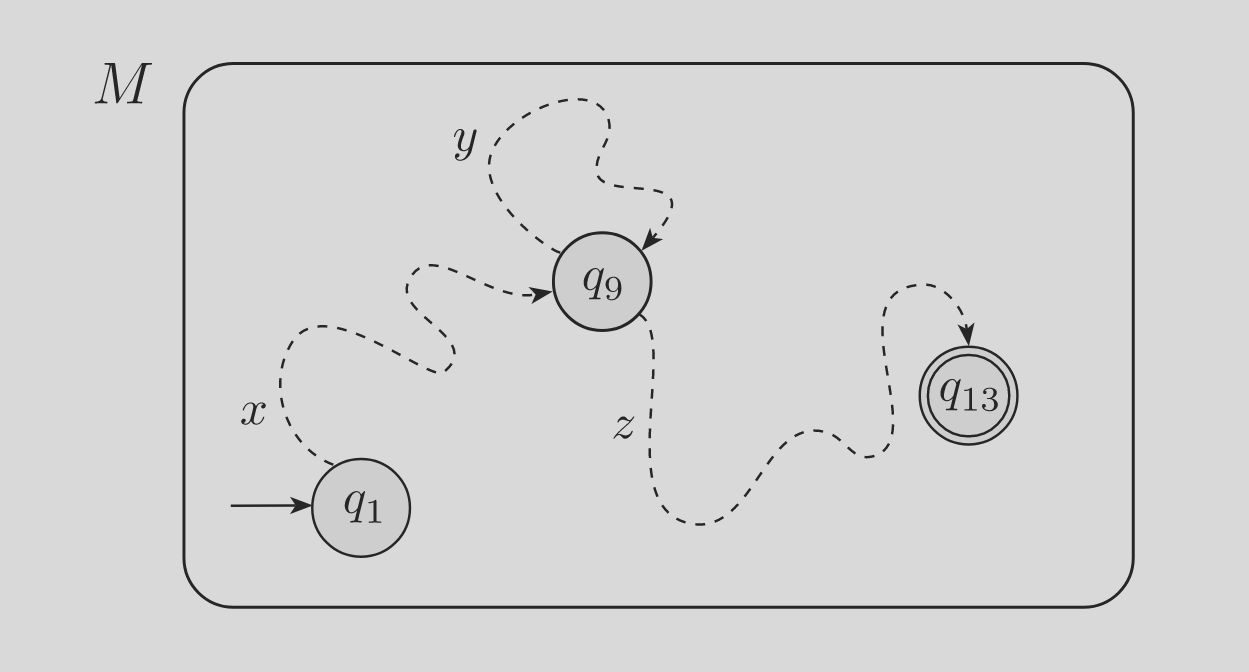
\includegraphics[scale=0.35]{../assets/pump-neg.png}
            \caption{L'automa $M$ descritto.}
        \end{figure}

    \end{proof}

    \begin{example}[Pumping lemma]
        Sia $B = \{\ttt 0 ^n \ttt 1 ^n \mid n \ge 0\}$ un linguaggio. TODO NON HO CAPITO
    \end{example}

    \chapter{Linguaggi e grammatiche context-free}

    \section{Grammatiche context-free}

    \subsection{Definizioni}

    \begin{frameddefn}[breakable]{Grammatica context-free}
        Una \tbf{grammatica context-free}, o CFG (\tit{Context-Free Grammar}) è una quadrupla $(V, \Sigma, R, S)$, dove

        \begin{itemize}
            \item $V$ è l'insieme delle \tbf{variabili}, un insieme \tit{finito}
            \item $\Sigma$ è l'insieme dei \tbf{terminali}, un insieme \tit{finito}, dove $\Sigma \cap V = \varnothing$
            \item $R$ è l'insieme delle \tbf{regole} o \tbf{produzioni}, un insieme \tit{finito}
            \item $S \in V$ è la \tbf{variabile iniziale}, ed è generalmente il primo simbolo della prima regola della grammatica
        \end{itemize}

        Le CFG sono della forma $$\left . \begin{array}{c} X \to Y \\ \vdots \end{array} \right .$$ dove $X, Y \in V$, e $X \to Y \in R$ è una regola della CFG.

        Una grammatica è un insieme di regole di sostituzione di stringhe, in grado di produrre quest'ultime a partire da una variabile iniziale, mediante una sequenza di scambi. In particolare, partendo dalla variabile iniziale, vengono sostituiti gli elementi alla sinistra del simbolo $\to$ di una certa regola in $R$, con quelli alla sua destra.

        Due regole $X \to Y, X \to Z \in R$ possono essere accorpate con $X \to Y | Z$. Siano $u, v, w$ stringhe di variabili in $V$, e $A \to w \in R$; si dice che $uAv$ \tbf{produce} $uwv$, denotato con $uAv \implies uwv$. Se $u = v$, oppure esistono stringhe $u_1, \ldots, u_k$ con $k \ge 0$ tali che $$u \implies u_1 \implies \ldots \implies u_k \implies v$$ si dice che $u$ \tbf{deriva} $v$, denotato con $u \ximplies{*} v$.
    \end{frameddefn}

    \begin{example}[CFG]
        \label{cfg ex}
        Un esempio di CFG è il seguente: $$\left . \begin{array}{c} A \to \ttt 0 A \ttt 1 \\ A \to B \\ B \to \ttt \# \end{array} \right .$$ In essa, si hanno: $$\left . \begin{array}{c} V := \{A, B\} \\ \Sigma := \{\ttt 0, \ttt 1, \ttt \# \} \\ S := A \in V \end{array} \right. $$

        Da essa, è possibile ottenere la stringa $\ttt{000\#111}$ attraverso le seguenti sostituzioni: $$A \implies \ttt 0 A \ttt 1 \implies \ttt{000}A\ttt{111} \implies \ttt{000}B\ttt{111} \implies \ttt{000\#111}$$
    \end{example}

    \begin{frameddefn}{Linguaggio di una grammatica}
        Data una grammatica $G$, il suo \tbf{linguaggio} è l'insieme delle stringhe che la grammatica $G$ è in grado di generare, ed è denotato con $L(G)$. In simboli, data una grammatica $G$, si ha che $$L(G) = \{w \in \Sigma ^* \mid S \ximplies{*} w\}$$

        Se $G$ è una CFG, allora $L(G)$ è detto \tbf{linguaggio context-free}, o CFL (\tit{Context-Free Language}).
    \end{frameddefn}

    \begin{example}[CFL]
        Si prenda in esame la CFG dell'\cref{cfg ex}, e sia essa $G$. Allora, in tale grammatica il linguaggio risulta essere $$L(G) = \{\ttt 0 ^n \ttt \# \ttt 1 ^n \mid n \ge 0\}$$
    \end{example}

    \begin{frameddefn}{Derivazione a sinistra}
        Sia $G$ una grammatica; una stringa si dice essere \tbf{derivata a sinistra} se è stata ottenuta applicando regole di $G$ sulle variabili più a sinistra disponibili.
    \end{frameddefn}

    \begin{example}[Derivazione a sinistra]
        TODO
    \end{example}

    \begin{frameddefn}{Ambiguità}
        Sia $G$ una grammatica; se esistono due stringhe $u, v$ con $u \neq v$, tali che esiste una terza stringa $z$ derivata a sinistra sia da $u$ che da $v$, si dice che $G$ genera $z$ \tbf{ambiguamente}; inoltre, $G$ si dice essere \tbf{ambigua} se genera stringhe ambiguamente.
    \end{frameddefn}

    \begin{frameddefn}{Linguaggi inerentemente ambigui}
        Un linguaggio si dice essere \tbf{inerentemente ambiguo} se non esistono grammatiche non ambigue che lo possano generare.
    \end{frameddefn}

    \begin{example}[Linguaggi inerentemente ambigui]
        TODO $\{\ttt a ^i \ttt b^j \ttt c^k \mid i = j \lor j = k\}$
    \end{example}

    \begin{frameddefn}{Forma normale di Chomsky}
        Una CFG $(V, \Sigma, R, S)$ è in \tbf{forma normale di Chomsky}, o CNF (\tit{Chomsky Normal Form}), se ogni regola è della forma $$\left . \begin{array}{c} A \to BC \\ A \to a \end{array} \right .$$ dove $$\left . \begin{array}{c} V := \{ A, B, C \} \\ \Sigma := \{ a\} \\ S := A \end{array} \right .$$ e la regola $S \to \varepsilon \in R$ è sempre permessa, chiamata \tbf{$\varepsilon$-regola}.

        Dunque, la CNF non permette di

        \begin{enumerate}[label=\roman*), font=\itshape]
            \item avere \tbf{regole unitarie}, ovvero regole della forma $A \to B$;
            \item avere regole della forma $X \to S \in R$ per qualche $X \in V$, ovvero avere $S$ alla destra del simbolo $\to$ di una regola.
        \end{enumerate}
    \end{frameddefn}

    \begin{framedthm}{CFL generati da CFG in CNF}
        Ogni CFL è generato da una CFG in forma normale di Chomsky.
    \end{framedthm}

    \begin{proof}
        Sia un CFL generato da una CFG $G = (V, \Sigma, R, S)$. Allora, è possibile rendere $G$ in CNF attraverso i seguenti passaggi:

        \begin{itemize}
            \item vengono aggiunte la variabile $S_0 \in V$, e la regola $S_0 \to S \in R$, in modo da non avere $S$ alla destra di nessuna regola in $R$;
            \item ogni regola $A \to \varepsilon \in R$ per qualche $A \in V - \{S\}$ viene rimossa da $R$, e successivamente per ogni regola della forma $X \to uAv \in R$ per qualche $X \in V$ e $u, v$ stringhe di variabili e terminali, viene aggiunta $X \to uv \in R$; inoltre, se $X \to A \in R$, allora viene aggiunta $X \to \varepsilon \in R$, solo se quest'ultima non era stata precedentemente rimossa;
            \item ogni regola unitaria $A \to B \in R$ viene rimossa, ed ogni regola $B \to u \in R$ per qualche stringa $u$ di variabili o terminali, viene aggiunta $A \to u \in R$, solo se questa non era una regola unitaria precedentemente rimossa;
            \item infine, ogni regola restante $A \to u_1 \ldots u_k$ con $k \ge 3$ e $u_1, \ldots, u_k$ stringhe di variabili o terminali viene rimpiazzata con le regole $$\left . \begin{array}{c} A \to u_1 A_1  \\ A_1 \to u_2 A_2 \\ A_2 \to u_3 A_3 \\ \vdots \\ A_{k - 2} \to u_{k - 1}u_k \end{array} \right .$$ e $A_1, \ldots, A_{k - 2} \in V$; inoltre, ogni terminale $u_i$ per ogni $i \in [1, k]$ viene rimpiazzato con la nuova varibile $U_i$, e viene aggiunta la regola TODO DA FINIRE
        \end{itemize}

    \end{proof}

    \section{Automi a pila}

    \subsection{Definizioni}

    \begin{frameddefn}{PDA}
        Un \tbf{PDA} (\tit{Pushdown Automaton}) è una sestupla $(Q, \Sigma, \Gamma, \delta, q_0, F)$, dove

        \begin{itemize}
            \item $Q$ è l'\tbf{insieme degli stati}, un insieme \tit{finito}
            \item $\Sigma$ è l'\tbf{alfabeto dell'automa}, un insieme \tit{finito}
            \item $\Gamma$ è l'\tbf{alfabeto dello stack} (o \tit{pila}), un insieme \tit{finito}
            \item $\func{\delta}{Q \times \Sigma_\varepsilon \times \Gamma_\varepsilon}{\powerset{(Q \times \Gamma_\varepsilon)}}$ è la \tbf{funzione di transizione}, che definisce la relazione tra gli stati
            \item $q_0 \in Q$ è lo \tbf{stato iniziale}
            \item $F \subseteq Q$ è l'\tbf{insieme degli stati accettanti}
        \end{itemize}

        dove $\Gamma_\varepsilon := \Gamma \cup \{ \varepsilon \}$.

        Un PDA è un NFA dotato di uno \tbf{stack} illimitato, che gli consente di riconoscere alcuni linguaggi non regolari, poiché in esso è in grado di porre i simboli che legge dalla stringa di input, di fatto implementando un sistema di \tit{memoria}.
        
        Si noti che la macchina può usare differenti alfabeti per il suo input e la sua pila, infatti la definizione formale vede due alfabeti distinti, $\Sigma$ e $\Gamma$ rispettivamente. Inoltre, $\Gamma_\varepsilon$ compare nel prodotto cartesiano del dominio di $\delta$, poiché il simbolo in cima allo stack del PDA è in grado di determinare anch'esso la mossa seguente dell'automa; a tal proposito, $\varepsilon \in \Gamma$ permette di ignorare il primo elemento della pila. In aggiunta, $\Gamma_\varepsilon$ compare anche all'interno dell'insieme potenza (si noti che un PDA è non deterministico) del codominio di $\delta$, al fine di poter decidere se si vuole salvare il simbolo letto all'interno dello stack o meno (tramite $\varepsilon \in \Gamma$).
    \end{frameddefn}

    \begin{example}[PDA]
        \label{pda ex}
        Un esempio di PDA $(Q, \Sigma, \Gamma, \delta, q_1, F)$ è il seguente:

        \begin{itemize}
            \item $Q = \{q_1, q_2, q_3, q_4\}$
            \item $\Sigma = \{ \ttt 0, \ttt 1 \}$
            \item $\Gamma = \{ \ttt 0, \ttt \$\}$
            \item $F = \{ q_1, q_4 \}$
        \end{itemize}

        e $\delta$ è data dalla seguente tabella di transizione:

        \centeredimage{0.3}{../assets/delta-pda-neg.png}{L'immagine rappresenta $\delta$ in forma tabellare.}
    \end{example}

    \begin{frameddefn}{Stringhe accettate (PDA)}
        Sia $M = (Q, \Sigma, \Gamma, \delta, q_0, F)$ un PDA, e sia $w = w_1\cdots w_n$ una stringa tale per cui $\forall i \in [1, n] \quad w_i \in \Sigma_\varepsilon$; allora, $M$ \tbf{accetta} $w$ se esistono una sequenza di stati $r_0, \ldots, r_n \in Q$ e una sequenza di stringhe $s_0, \ldots, s_n \in \Gamma ^*$ tali per cui

        \begin{itemize}
            \item $r_0 = q_0$
            \item $s_0 = \varepsilon$, ovvero, lo stack è inizialmente vuoto
            \item $\forall i \in [0, n - 1] \quad \exists a, b \in \Gamma_\varepsilon, t \in \Gamma^* \mid (r_{i + 1}, b) \in \delta(r_i, w_{i + 1}, a) \land \soe{l}{s_i = at \\ s_{i +1} = bt}$, ovvero, $M$ si muove correttamente in base allo stato, al simbolo nello stack, ed al prossimo simbolo di input; si noti che le stringhe $s_0, \ldots, s_n$ rappresentano di fatto il contenuto dello stack che $M$ ha su un ramo accettante della computazione, infatti $s_i = at$ diventa $s_{i + 1} = bt$ con l'iterazione successiva, dunque $a$ è stato sostituito con $b$ in cima alla pila
            \item $r_n \in F$
        \end{itemize}
    \end{frameddefn}

    \begin{example}[Linguaggi riconosciuti da un PDA]
        \label{pda ex 2}
        Si prenda in considerazione il PDA descritto nell'\cref{pda ex}, e sia questo $M$. Il seguente è il suo diagramma di stato:

        \begin{figure}[H]
            \centering
            \begin{tikzpicture}[->,>=stealth,shorten >=1pt,auto,node distance=3cm,thick,main node/.style={scale=0.9,circle,draw,font=\sffamily\normalsize}]
                \node[initial,state,accepting] (1) {$q_1$};
                \node[state] (2) [right of=1] {$q_2$};
                \node[state] (3) [below of=2] {$q_3$};
                \node[state,accepting] (4) [below of=1] {$q_4$};
     
                \path[every node/.style={font=\sffamily\small}]
                    (1) edge node {$\varepsilon, \varepsilon \to \ttt \$$} (2)
                    (2) edge [loop above] node {$\ttt 0, \varepsilon \to \ttt 0$} (2)
                    (2) edge node {$\ttt 1, \ttt 0 \to \varepsilon$} (3)
                    (3) edge [loop below] node {$\ttt 1, \ttt 0 \to \varepsilon$} (3)
                    (3) edge node {$\varepsilon, \ttt \$ \to \varepsilon$} (4)
                 ;
             \end{tikzpicture}
             \caption{Il PDA $M$.}
        \end{figure}

        In questo diagramma, la notazione $\ttt a, \ttt b \to \ttt c$ presente sugli archi sta ad indicare che se viene letto il simbolo $\ttt a$ dall'input, $M$ può sostituire $\ttt b$, se in cima al suo stack (attraverso un'operazione di \tit{pop}) con $\ttt c$ (mediante un'operazione di \tit{push}). Si noti che ognuno dei simboli può essere $\varepsilon$, e dunque

        \begin{itemize}
            \item $\varepsilon, \ttt b \to \ttt c$ sta a significare che il ramo viene eseguito senza attendere alcun simbolo di input (si noti l'\cref{nfa exec} per il non determinismo)
            \item $\ttt a, \varepsilon \to \ttt c$ sta a significare che viene eventualmente effettuato solamente il \tit{push} di $\ttt c$ nello stack
            \item $\ttt a, \ttt b \to \varepsilon$ sta a significare che viene eventualmente effettuato solamente il \tit{pop} di $\ttt b$ dallo stack
        \end{itemize}

    \end{example}

    \begin{framedobs}[label={pda empty stack}]{Stack vuoto (PDA)}
        Un PDA non è in grado di controllare se il suo stack è vuoto, ma è possibile ottenere questo effetto come segue: si prenda in esame il PDA $M$ dell'\cref{pda ex 2}; è importante notare che esso utilizza il simbolo $\ttt \$$ per capire se lo stack è vuoto o meno, poiché viene inserito sin dall'inizio (si osservi l'etichetta $\varepsilon, \varepsilon \to \ttt \$$ sull'arco $(q_1, q_2)$), e dunque se viene letto $\ttt \$$ in cima allo stack, $M$ sa che quello è l'unico elemento contenuto al suo interno, e lo stack è di fatto vuoto.
    \end{framedobs}

    \begin{framedobs}{Fine dell'input (PDA)}
        Un PDA non è in grado di controllare se è stata raggiunga la fine della stringa di input, ma è possibile ottenere questo effetto come segue: si prenda in esame il PDA $M$ dell'\cref{pda ex 2}; è importante notare che esso può sapere se è stata raggiunta la fine della stringa di input, poiché lo stato accettante $q_4$ può essere eventualmente raggiunto solamente alla lettura di $\varepsilon$ e nel momento in cui è possibile rimuovere $\ttt \$$ dallo stack (si noti l'\cref{pda empty stack}).
    \end{framedobs}

    \begin{framedmeth}[breakable]{Trasformare CFG in DPA}
        \label{cfg into pda}
        TODO DA RILEGGERE E FINIRE

        Si vuole introdurre una notazione per l'inserimento di un'intera stringa all'interno dello stack di $P$, accorpando tale operazione in un solo passo dell'automa. Infatti, con la notazione

        \begin{figure}[H]
            \centering
            \begin{tikzpicture}[->,>=stealth,shorten >=1pt,auto,node distance=3cm,thick,main node/.style={scale=0.9,circle,draw,font=\sffamily\normalsize}]
                \node[state] (1) {$q$};
                \node[state] (2) [right of=1] {$r$};
     
                \path[every node/.style={font=\sffamily\small}]
                    (1) edge node {$a, s \to xyz$} (2)
                 ;
             \end{tikzpicture}
             \caption{Un PDA che inserisce una stringa nello stack.}
        \end{figure}

        presente sull'arco $(q, r)$, per qualche $a \in \Sigma_\varepsilon, s \in \Gamma_\varepsilon$, si sottointende l'inserimento di stati aggiuntivi in grado di realizzare l'operazione seguente:

        \begin{figure}[H]
            \centering
            \begin{tikzpicture}[->,>=stealth,shorten >=1pt,auto,node distance=3cm,thick,main node/.style={scale=0.9,circle,draw,font=\sffamily\normalsize}]
                \node[state] (1) {$q$};
                \node[state] (2) [right of=1] {$q_1$};
                \node[state] (3) [right of=2] {$q_2$};
                \node[state] (4) [right of=3] {$r$};
     
                \path[every node/.style={font=\sffamily\small}]
                    (1) edge node {$a, s \to z$} (2)
                    (2) edge node {$\varepsilon, \varepsilon \to y$} (3)
                    (3) edge node {$\varepsilon, \varepsilon \to x$} (4)
                 ;
             \end{tikzpicture}
             \caption{La formalizzazione del PDA precedente.}
        \end{figure}

        In simboli, la notazione $(r, u) \in \delta(q, a, s)$, per qualche stringa $u := u_1, \ldots, u_n$ sottoindente la seguente: $$\begin{array}{c} (q_1, u_n) \in \delta(q, a, s) \\ \delta(q_1, \varepsilon, \varepsilon) := \{(q_2, u_{n - 1}) \}\\ \vdots \\ \delta(q_{n - 1}, \varepsilon, \varepsilon) := \{(r, u_1)\} \end{array}$$

        Sia $G = (V, \Sigma, R, S)$ una CFG, e sia $E$ l'insieme di stati tali da realizzare l'accorpamento appena descritto, relativo alla grammatica $G$; si vuole dunque costruire un PDA $$P = (\{q_0, q', q\} \cup E, \Sigma, \Gamma, \delta, q_0, \{q\})$$ che sia equivalente a $G$, ed è possibile realizzarlo come segue:

        \begin{itemize}
            \item $\delta(q_0, \varepsilon, \varepsilon) := \{(q', S \ttt \$) \}$, ovvero, viene inserito $\ttt \$$ come marcatore nello stack di $P$ (si noti l'\cref{pda empty stack}), e successivamente la stringa iniziale $S$ di $G$;
            \item $\forall A \in V \quad \delta(q', \varepsilon, A) := \{ (q', w) \mid A \to w \in R\}$ dove $w$ è una stringa di $G$; con questa operazione, se viene incontrata una variabile $A$ sulla cima dello stack di $P$, viene scelta una delle regole di $G$ in grado di sostituire $A$, non deterministicamente;
            \item $\forall a \in \Gamma_\varepsilon \quad \delta(q', a, a) := \{ (q', \varepsilon) \}$ TODO NON HO CAPITO IL PERCHÉ
            \item $\delta(q', \varepsilon, \ttt \$) := \{(q, \varepsilon) \}$, ovvero, se $\ttt \$$ è in cima allo stack, allora $P$ entra nello stato accettante, in modo tale da accettare l'input solo se quest'ultimo è stato completamente letto
        \end{itemize}

        \begin{figure}[H]
            \centering
            \begin{tikzpicture}[->,>=stealth,shorten >=1pt,auto,node distance=3cm,thick,main node/.style={scale=0.9,circle,draw,font=\sffamily\normalsize}]
                \node[initial,state] (1) {$q_0$};
                \node[state] (2) [right of=1] {$q'$};
                \node[state,accepting] (3) [right of=2] {$q$};
     
                \path[every node/.style={font=\sffamily\small}]
                    (1) edge node {$\varepsilon, \varepsilon \to S \ttt \$$} (2)
                    (2) edge [loop above] node {$(\varepsilon, A \to \varepsilon), (a, a \to \varepsilon a)$} (2)
                    (2) edge node {$\varepsilon, \ttt \$ \to \varepsilon$} (3)
                 ;
             \end{tikzpicture}
             \caption{Il PDA $P$ appena costruito.}
        \end{figure}

    \end{framedmeth}

    \begin{framedthm}{CFL e PDA}
        Un linguaggio è context-free se e solo se esiste un PDA che lo riconosce.
    \end{framedthm}

    \proofiff{
        Sia $A$ un CFL, e sia $G$ la CFG che lo genera (per definizione); allora, utilizzando il \cref{cfg into pda}, è possibile trasformare $G$ in un PDA ad essa equivalente, e dunque segue la tesi.
    }{
        TODO
    }

    \section{Linguaggi non context-free}

    \subsection{Pumping lemma}

    \begin{framedlem}{Pumping lemma (CFL)}
        Sia $A$ un CFL; allora, esiste un $p \in \N$, detto \tbf{lunghezza del pumping}, tale che per ogni stringa $s \in A$ tale per cui $|s| \ge p$, esistono 5 stringhe $u, v, x, y, z \in A \mid s = uvxyz$ soddisfacenti le seguenti condizioni:

        \begin{itemize}
            \item $\forall i \ge 0 \quad uv^ixy^iz \in A$
            \item $|vy| > 0$ (o, equivalentemente, $v \neq \varepsilon \lor y \neq \varepsilon$)
            \item $|vxy| \le p$
        \end{itemize}
    \end{framedlem}

    \begin{proof}
        Poiché $A$ è un CFG, allora per definizione esiste una CFG $G$ che lo genera. TODO
    \end{proof}
    
    \section{Linguaggi context-free deterministici}

    \subsection{Automi a pila deterministici}

    \begin{frameddefn}{DPDA}
        Un \tbf{DPDA} (\tit{Deterministic Pushdown Automaton}) è una sestupla $(Q, \Sigma, \Gamma, \delta, q_0, F)$, dove

        \begin{itemize}
            \item $Q$ è l'\tbf{insieme degli stati}, un insieme \tit{finito}
            \item $\Sigma$ è l'\tbf{alfabeto} dell'automa, un insieme \tit{finito}
            \item $\Sigma$ è l'\tbf{alfabeto dello stack}, un insieme \tit{finito}
            \item $\func{\delta}{Q \times \Sigma_\varepsilon \times \Gamma_\varepsilon}{(Q \times \Gamma_\varepsilon) \cup \{\emptyset \}}$ è la \tbf{funzione di transizione}, che definisce la relazione tra gli stati
            \item $q_0 \in Q$ è lo \tbf{stato iniziale}
            \item $F \subseteq Q$ è l'\tbf{insieme degli stati accettanti}
        \end{itemize}

        Si noti che, nonostante l'automa sia deterministico, un DPDA è in grado di lavorare con $\varepsilon$.

        Poiché un DPDA è la controparte deterministica di un PDA, $\delta$ deve verificare la seguente condizione: per ogni $q \in Q, a \in \Sigma, x \in \Gamma$, solo uno tra $\delta(q, a, x)$, $\delta(q, a, \varepsilon)$, $\delta(q, \varepsilon, x)$ e $\delta(q, \varepsilon, \varepsilon)$ è diverso da $\emptyset$. In particolare, $\delta(q, \varepsilon, x)$ è detta \tbf{$\varepsilon$-mossa} di \tbf{$\varepsilon$-input}, mentre $\delta(q, a, \varepsilon)$ è detta \tbf{$\varepsilon$-mossa} di \tbf{$\varepsilon$-pila}.

        Se la pila del DPDA è vuota, questo può fare mosse solo se $\delta$ specifica una mossa che elimina $\varepsilon$, altrimenti non sono previste mosse lecite ed il DPDA rifiuta l'input senza leggerne il resto; questa situazione viene detta \tit{hanging}. Inoltre, si verifica un rifiuto anche se il DPDA effettua una sequenza infinita di mosse $\varepsilon$-input, senza leggere l'input oltre un certo punto; questa situazione viene detta \tit{looping}.
    \end{frameddefn}

    \begin{framedlem}{DPDA equivalenti}
        Ogni DPDA ha un DPDA equivalente che legge sempre l'intera stringa di input; dunque non si presenta mai né \tit{hanging} né \tit{looping}.
    \end{framedlem}

    \begin{proof}
        Sia $P = (Q, \Sigma, \Gamma, \delta, q_0, F)$ un DPDA; in primo luogo, $q_0$ viene rimpiazzato con un nuovo stato iniziale $q_{\mathrm{start}}$; successivamente, $q_{\mathrm{reject}}$ viene aggiunto ad $F$, ed inoltre, per ogni $r \in Q, a \in \Sigma_\varepsilon, x, y \in \Gamma_\varepsilon$ si effettuano le seguenti variazioni:

        \begin{itemize}
            \item per ogni $q \in Q$ si aggiunge uno stato $q_\mathrm{a}$, ed inoltre $$\forall q \in Q \quad \delta(q, \varepsilon, x) = (r, y) \implies \delta(q_\mathrm{a}, \varepsilon, x) := (r_\mathrm{a}, y)$$ inoltre $$q \in F \implies \delta(q, \varepsilon, x) := (r_\mathrm{a}, y)$$
        \end{itemize}

        TODO DA FINIRE NON HA NESSUN SENSO QUESTA DIMOSTRAZIONE
    \end{proof}

    \begin{frameddefn}{DCFL}
        Sia $M$ un DPDA, e sia $A$ il linguaggio che riconosce; allora, $A$ è detto \tbf{DCFL} (\tit{Deterministic Context-Free Language}).
    \end{frameddefn}

\end{document}
